\section{Giới hạn của hàm số}
\setcounter{dang}{0}
\subsection{Tóm tắt lý thuyết}
\begin{tomtat}
	\subsubsection{Giới hạn hữu hạn của hàm số tại một điểm}
	
	\begin{dn}
		Cho điểm $ x_0 $ thuộc khoảng $ K $ và hàm số $ y=f(x) $ xác định trên $ K $ hoặc $ K\setminus\{x_0\} $.\\
		Ta nói hàm số $ y=f(x) $ \textbf{\textit{có giới hạn hữu hạn}} là số $ L $ khi $ x $ dần tới $ x_0 $ nếu với dãy số $ (x_n) $ bất kì, $ x_n\in K\setminus\{x_0\} $ và $ x_n \to x_0 $ thì $ f(x_n)\to L $, kí hiệu $ \lim \limits_{x \to x_0} f(x) =L$ hay $ f(x)\to L $ khi $ x\to x_0 $.
	\end{dn}
	
	\begin{note} 
		$ \lim \limits_{x \to x_0} x=x_0 $; \quad $ \lim \limits_{x \to x_0} c=c $ ($ c $ là hằng số).
	\end{note} 
	\subsubsection{Các phép toán về giới hạn hữu hạn của hàm số}
	\begin{enumerate}
		\item Cho $ \lim \limits_{x \to x_0} f(x) =L$ và $ \lim \limits_{x \to x_0} g(x)=M $. Khi đó:
		\begin{itemize}
			\item $ \lim \limits_{x \to x_0} [f(x)+g(x)]=L+M $;
			\item $ \lim \limits_{x \to x_0} [f(x)-g(x)]=L-M $;
			\item $ \lim \limits_{x \to x_0} [f(x)\cdot g(x)]=L\cdot M $;
			\item $ \lim \limits_{x \to x_0} \dfrac{f(x)}{g(x)}=\dfrac{L}{M} $ (với $ M\neq 0 $).			
		\end{itemize}
		\item Nếu $ f(x)\geq 0 $ và $ \lim \limits_{x \to x_0} f(x) =L$ thì $ L\geq 0 $ và $ \lim \limits_{x \to x_0} \sqrt{f(x)}=\sqrt{L} $.\\
		(Dấu của $ f(x) $ được xét trên khoảng tìm giới hạn, $ x\neq x_0 $).
	\end{enumerate}
	\begin{note} 
		\indent
		\begin{enumerate}
			\item $ \lim \limits_{x \to x_0} x^k=x_0^k $, $ k $ là số nguyên dương;
			\item $ \lim \limits_{x \to x_0} [cf(x)]=c\lim \limits_{x \to x_0} f(x) $ ($ c\in \mathbb{R} $, nếu tồn tại $ \lim \limits_{x \to x_0} f(x) \in \mathbb{R}$).
		\end{enumerate}
	\end{note} 
	
	\subsubsection{Giới hạn một phía}
	\begin{dn}
		\
		\begin{itemize}
			\item Cho hàm số $ y=f(x) $ xác định trên khoảng $ (x_0;b) $.\\
			Ta nói hàm số $ y=f(x) $ \textbf{\textit{có giới hạn bên phải}} là số $ L $ khi $ x $ dần tới $ x_0 $ nếu với dãy số $ (x_n) $ bất kì, $ x_0<x_n<b $ và $ x_n\to x_0 $ thì $ f(x_n)\to L $, kí hiệu $ \lim \limits_{x \to x_0^+} f(x) =L$.
			\item Cho hàm số $ y=f(x) $ xác định trên khoảng $ (a;x_0) $.\\
			Ta nói hàm số $ y=f(x) $ \textbf{\textit{có giới hạn bên trái}} là số $ L $ khi $ x $ dần tới $ x_0 $ nếu với dãy số $ (x_n) $ bất kì, $ a<x_n<x_0 $ và $ x_n\to x_0 $ thì $ f(x_n)\to L $, kí hiệu $ \lim \limits_{x \to x_0^-} f(x) =L$.
		\end{itemize}
	\end{dn}
	\begin{note} 
		\begin{enumerate}
			\item Ta thừa nhận các kết quả sau:
			\begin{itemize}
				\item $ \lim \limits_{x \to x_0^+} f(x)=L$ và $ \lim \limits_{x \to x_0^-} f(x)=L $ khi và chỉ khi $ \lim \limits_{x \to x_0} f(x) =L$;
				\item Nếu $ \lim \limits_{x \to x_0^+} f(x)\neq \lim \limits_{x \to x_0^-} f(x)$ thì không tồn tại $ \lim \limits_{x \to x_0} f(x) $.
			\end{itemize}
			\item Các phép toán về giới hạn hữu hạn của hàm số ở Mục 2 vẫn đúng khi ta thay $ x\to x_0 $ bằng $ x\to x_0^+ $ hoặc $ x\to x_0^- $.
		\end{enumerate}
	\end{note}
	
	\subsubsection{Giới hạn hữu hạn của hàm số tại vô cực}
	\begin{dn}
		\
		\begin{itemize}
			\item Cho hàm số $ y=f(x) $ xác định trên khoảng $ (a;+\infty) $.\\
			Ta nói hàm số $ y=f(x) $ \textbf{\textit{có giới hạn hữu hạn}} là số $ L $ khi $ x \to +\infty  $ nếu với dãy số $ (x_n) $ bất kì, $ x_n>a $ và $ x_n\to +\infty $ thì $ f(x_n)\to L $, kí hiệu $ \lim \limits_{x \to +\infty} f(x) =L$ hay $ f(x) \to L $ khi $ x\to +\infty $.
			\item Cho hàm số $ y=f(x) $ xác định trên khoảng $ (-\infty;a) $.\\
			Ta nói hàm số $ y=f(x) $ \textbf{\textit{có giới hạn hữu hạn}} là số $ L $ khi $ x \to -\infty $ nếu với dãy số $ (x_n) $ bất kì, $ x_n<a $ và $ x_n\to -\infty $ thì $ f(x_n)\to L $, kí hiệu $ \lim \limits_{x \to -\infty} f(x) =L$ hay $ f(x)\to L $ khi $ x\to -\infty $.
		\end{itemize}
	\end{dn}
	\begin{note}
		\begin{enumerate}
			\item Với $ c $ là hằng số và $ k $ là  số nguyên dương, ta luôn có:
			$$\lim \limits_{x \to \pm \infty} c=c\quad \text{và} \quad \lim \limits_{x \to \pm \infty} \dfrac{c}{x^k}=0.$$
			\item Các phép toán trên giới hạn hàm số ở Mục 2 vẫn đúng khi thay $ x\to x_0 $ bằng $ x\to +\infty $ hoặc $ x\to -\infty $.
		\end{enumerate}
	\end{note}
	
	\subsubsection{Giới hạn vô cực của hàm số tại một điểm}
	
	\begin{dn}
		Cho hàm số $ y=f(x) $ xác định trên khoảng $ (x_0;b) $.
		\begin{itemize}
			\item 
			Ta nói hàm số $ y=f(x) $ \textbf{\textit{có giới hạn bên phải}} là $ +\infty $ khi $ x $ dần tới $ x_0 $ về bên phải nếu với dãy số $ (x_n) $ bất kì, $ x_0<x_n<b $ và $ x_n\to x_0 $ thì $ f(x_n)\to +\infty $, kí hiệu $ \lim \limits_{x \to x_0^+} f(x) =+\infty$ hay $ f(x)\to +\infty $ khi $ x \to x_0^+ $.
			\item Ta nói hàm số $ y=f(x) $ \textbf{\textit{có giới hạn bên phải}} là  $ -\infty $ khi $ x $ dần tới $ x_0 $ về bên phải nếu với dãy số $ (x_n) $ bất kì, $ x_0<x_n<b $ và $ x_n\to x_0 $ thì $ f(x_n)\to -\infty $, kí hiệu $ \lim \limits_{x \to x_0^+} f(x) =-\infty$ hay $ f(x)\to -\infty $ khi $ x\to x_0^+ $.
		\end{itemize}
	\end{dn}
	
	\begin{note}
		\begin{enumerate}
			\item Các giới hạn $ \lim \limits_{x \to x_0^-} f(x)=+\infty $, $ \lim \limits_{x \to x_0^-} f(x)=-\infty $, $ \lim \limits_{x \to +\infty} f(x)=+\infty $, $ \lim \limits_{x \to +\infty} f(x)=-\infty $, $ \lim \limits_{x \to -\infty} f(x)=+\infty $, $ \lim \limits_{x \to -\infty} f(x)=-\infty $ được định nghĩa như trên.
			\item Ta có các giới hạn thường dùng như sau:
			\begin{itemize}
				\item $ \lim \limits_{x \to a^+} \dfrac{1}{x-a}=+\infty $ và $ \lim \limits_{x \to a^-}\dfrac{1}{x-a}=-\infty $ ($ a\in \mathbb{R} $);
				\item $ \lim \limits_{x \to +\infty}x^k=+\infty $ với $ k $ nguyên dương;
				\item $ \lim \limits_{x \to -\infty}x^k=+\infty $ với $ k $ là số chẵn;
				\item $ \lim \limits_{x \to -\infty}x^k=-\infty $ với $ k $ là số lẻ.
			\end{itemize}
			\item Các phép toán trên giới hạn hàm số của Mục 2 chỉ áp dụng được khi tất cả các hàm số được xét có giới hạn hữu hạn. Với giới hạn vô cực, ta có một số quy tắc sau đây.\\
			Nếu $ \lim \limits_{x \to x_0^+} f(x)=L\neq 0 $ và $ \lim \limits_{x \to x_0^+} g(x)=+\infty $ (hoặc $ \lim \limits_{x \to x_0^+} g(x)=-\infty $) thì $ \lim \limits_{x \to x_0^+}[f(x)\cdot g(x)] $ được tính theo quy tắc cho bởi bảng sau:
			\begin{center}
				\begin{tabular}{|c|c|c|}
					\hline 
					$ \lim \limits_{x \to x_0^+} f(x) $	& $  \lim \limits_{x \to x_0^+} g(x) $&$ \lim \limits_{x \to x_0^+} [f(x)\cdot g(x)] $  \\ 
					\hline 
					$ L>0 $	&$ +\infty $  &$ +\infty $  \\ 
					\hline 
					$ L>0 $	&$ -\infty $ &$ -\infty $  \\ 
					\hline 
					$ L<0 $&  $ +\infty $&  $ -\infty $\\ 
					\hline 
					$ L<0 $& $ -\infty $ &$ +\infty $  \\ 
					\hline 
				\end{tabular} 
			\end{center}
			Các quy tắc trên vẫn đúng khi thay $ x_0^+ $ thành $ x_0^- $ (hoặc $ +\infty $, $ -\infty $).
		\end{enumerate}
	\end{note}
\end{tomtat}

\subsection{Các dạng toán thường gặp}
\begin{dang}{Thay số trực tiếp}
\end{dang}
\subsubsection{Ví dụ minh hoạ}
\begin{vd}%[1K5YF-2]
	Tính các giới hạn sau
	\begin{listEX}[2]
		\item $ \lim \limits_{x \to 1} (x^2-4x+2)$;
		\item $ \lim \limits_{x \to 2} \dfrac{3x-2}{2x+1}$.
	\end{listEX}
	\loigiai{
		\begin{enumerate}[a)]
			\item $ \lim \limits_{x \to 1} (x^2-4x+2)=\lim \limits_{x \to 1} x^2-\lim \limits_{x \to 1} (4x)+\lim \limits_{x \to 1} 2=1^2-4\lim \limits_{x \to 1} x+2=1-4\cdot 1+2=-1$;
			\item $ \lim \limits_{x \to 2} \dfrac{3x-2}{2x+1}=\dfrac{\lim \limits_{x \to 2} (3x-2)}{\lim \limits_{x \to 2} (2x+1)}=\dfrac{3\lim \limits_{x \to 2} x-2}{2\lim \limits_{x \to 2} x+1}=\dfrac{3 \cdot 2-2}{2\cdot 2+1}=\dfrac{4}{5}$.
		\end{enumerate}
	}
\end{vd}

\begin{vd}%[1K5YF-2]
	Tìm các giới hạn sau
	\begin{enumEX}[a)]{2}
		\item $\lim\limits_{x\to 3} \sqrt{\dfrac{x^2}{x^3-x-6}}$.
		\item $\lim\limits_{x\to -2} \sqrt[3]{\dfrac{2x^4+3x+2}{x^2-x+2}}$.
	\end{enumEX}
	\loigiai{
		\begin{enumerate}[a)]
			\item $\lim\limits_{x\to 3} \sqrt{\dfrac{x^2}{x^3-x-6}}$; do $\lim\limits_{x\to 3} \dfrac{x^2}{x^3-x-6}=\dfrac{3^2}{3^3-3-6}=\dfrac{1}{2}>0$ \\
			$ \Rightarrow \lim\limits_{x\to 3} \sqrt{\dfrac{x^2}{x^3-x-6}}=\sqrt{\dfrac{1}{2}}=\dfrac{\sqrt{2}}{2}$.
			\item $\lim\limits_{x\to -2} \sqrt[3]{\dfrac{2x^4+3x+2}{x^2-x+2}}$; do $\lim\limits_{x\to -2} \dfrac{2x^4+3x+2}{x^2-x+2}=\dfrac{7}{2} \Rightarrow \lim\limits_{x\to -2} \sqrt[3]{\dfrac{2x^4+3x+2}{x^2-x+2}}=\sqrt[3]{\dfrac{7}{2}}=\dfrac{\sqrt[3]{28}}{2}$. 
		\end{enumerate}
	}
\end{vd}


\begin{vd}%[1K5YF-2]
	Cho $f(x)$ là một đa thức thỏa mãn $\displaystyle\lim\limits_{x\to 1}\dfrac{f(x)-16}{x-1}=24$. Tính giới hạn sau $$\displaystyle\lim\limits_{x\to 1}\dfrac{f(x)-16}{\left({x-1}\right)\left(\sqrt{2f(x)+4}+6\right)}.$$
	\loigiai{
		Vì $\displaystyle\lim\limits_{x\to 1}\dfrac{f(x)-16}{x-1}=24$ nên $f(1)=16.$ Khi đó
		$$ \lim\limits_{x\to 1}\dfrac{f(x)-16}{\left({x-1}\right)\left(\sqrt{2f(x)+4}+6\right)} =\frac{1}{12}\cdot \lim\limits_{x\to 1}\dfrac{f(x)-16}{x-1}=2.$$
	}
\end{vd}
% \subsubsection{Bài tập rèn luyện}
% % \subsubsection{Bài tập tự luận}
% \begin{bt}%[1K5YF-2]
% 	Tính các giới hạn sau:
% 	\begin{listEX}[2]
% 		\item $ \lim \limits_{x \to -2} (x^2+5x-2)$;
% 		\item $ \lim \limits_{x \to 1} \dfrac{x^2-1}{x-1}$.
% 	\end{listEX}
% 	\loigiai{
% 		\begin{enumerate}
% 			\item $ \lim \limits_{x \to -2} (x^2+5x-2)=(\lim \limits_{x \to -2} x)^2+\lim \limits_{x \to -2} (5x)-\lim \limits_{x \to -2} 2=(-2)^2+5\cdot (-2)-2=-8$.
% 			\item $ \lim \limits_{x \to 1} \dfrac{x^2-1}{x-1}=\lim \limits_{x \to 1} \dfrac{(x-1)(x+1)}{(x-1)}=\lim \limits_{x \to 1} (x+1)=\lim \limits_{x \to 1} x+1=1+1=2$.
% 		\end{enumerate}
% 	}
% \end{bt}

% \begin{bt}%[1K5YF-2]
% 	Tính các giới hạn sau
% 	\begin{enumEX}[a)]{2}
% 		\item $\lim\limits_{x\to -1} (3x^2-2x+1)$.
% 		\item $\lim\limits_{x\to 2} \dfrac{(x^3-3x)(x+1)}{x^2+3}$.
% 	\end{enumEX}
% 	\loigiai{
% 		\begin{enumerate}[a)]
% 			\item $\lim\limits_{x\to -1} (3x^2-2x+1)=3\lim\limits_{x\to -1} x^2-2\lim\limits_{x\to -1} x+\lim\limits_{x\to -1} 1=3{(1)}^2-2\cdot 1+1=2$.
% 			\item Do $\lim\limits_{x\to 2} (x^2+3)=2^2+3=7\ne 0$ và\\ $$\lim\limits_{x\to 2} (x^3-3x)(x+1)=\lim\limits_{x\to 2} (x^3-3x)\cdot \lim\limits_{x\to 2} (x+1)=(2^3-3\cdot 2)\cdot (2+1)=6$$
% 			Nên $\lim\limits_{x\to 2} \dfrac{(x^3-3x)(x+1)}{x^2+3}=\dfrac{6}{7}$.
% 		\end{enumerate}
% 	}
% \end{bt}

% \begin{bt}%[1K5YF-2]
% 	Tìm các giới hạn sau
% 	\begin{enumEX}[a)]{2}
% 		\item $\lim\limits_{x\to 2} \sqrt{\dfrac{2}{x^2-x+3}}$.
% 		\item $\lim\limits_{x\to -3} \sqrt[3]{\dfrac{-5}{x^2+x-12}}$.
% 	\end{enumEX}
% 	\loigiai{
% 		\begin{enumerate}[a)]
% 			\item $\lim\limits_{x\to 2} \sqrt{\dfrac{x}{x^2-x+3}}$; do $\lim\limits_{x\to 2} \dfrac{2}{x^2-x+3}=\dfrac{2}{2^2-2+3}=\dfrac{2}{5}>0$ \\
% 			$ \Rightarrow \lim\limits_{x\to 2} \sqrt{\dfrac{2}{x^2-x+3}}=\sqrt{\dfrac{2}{5}}=\dfrac{\sqrt{10}}{5}$.
% 			\item $\lim\limits_{x\to -3} \sqrt[3]{\dfrac{-5}{x^2+x-12}}$; do $\lim\limits_{x\to -3} \dfrac{-5}{x^2+x-12}=\dfrac{5}{6} \Rightarrow \lim\limits_{x\to -3} \sqrt[3]{\dfrac{-5}{x^2+x-12}}=\sqrt[3]{\dfrac{5}{6}}=\dfrac{\sqrt[3]{180}}{6}$. 
% 		\end{enumerate}
% 	}
% \end{bt} 

% \begin{bt}%[1K5YF-2]
% 	Cho $f(x)=x-1$ và $g(x)=x^{3}$. Tính các giới hạn sau:
% 	\begin{enumerate}
% 		\item $\lim \limits_{x \rightarrow 1}[3 f(x)-g(x)]$.
% 		\item $\lim \limits_{x \rightarrow 1} \dfrac{[f(x)]^{2}}{g(x)}$.
% 	\end{enumerate}
% 	\loigiai{Ta có $\lim \limits_{x \rightarrow 1} f(x)=\lim \limits_{x \rightarrow 1}(x-1)=\lim \limits_{x \rightarrow 1} x-\lim \limits_{x \rightarrow 1} 1=1-1=0$. Mặt khác, ta thấy $\lim \limits_{x \rightarrow 1} g(x)=\lim \limits_{x \rightarrow 1} x^{3}=1$.
% 		\begin{enumerate}
% 			\item Ta có
% 			$$
% 			\lim \limits_{x \rightarrow 1}[3 f(x)-g(x)]=\lim \limits_{x \rightarrow 1}[3 f(x)]-\lim \limits_{x \rightarrow 1} g(x)=\lim \limits_{x \rightarrow 1} 3 \cdot \lim \limits_{x \rightarrow 1} f(x)-\lim \limits_{x \rightarrow 1} g(x)=3 \cdot 0-1=-1 .
% 			$$
% 			\item  Ta có
% 			$$
% 			\lim \limits_{x \rightarrow 1} \dfrac{[f(x)]^{2}}{g(x)}=\dfrac{\lim \limits_{x \rightarrow 1}[f(x)]^{2}}{\lim \limits_{x \rightarrow 1} g(x)}=\dfrac{\lim \limits_{x \rightarrow 1} f(x) \cdot \lim \limits_{x \rightarrow 1} f(x)}{\lim \limits_{x \rightarrow 1} g(x)}=\dfrac{0}{1}=0.
% 			$$
% 	\end{enumerate}}
% 	\subsubsection{Bài tập trắc nghiệm}
% \end{bt}
\subsubsection{Câu hỏi trắc nghiệm}
\Opensolutionfile{ans}[ans/ans-1K5-2-Dang1]
\begin{ex}%[1T3Y2-1]
	Biết $\lim\limits_{x \to +\infty}f(x)=m$, $\lim\limits_{x \to +\infty}g(x)=n$. Tính $\lim\limits_{x \to +\infty}\left[f(x)+g(x)\right]$.
	\choice
	{\True $m+n$}
	{$m-n$}
	{$mn$}
	{$\dfrac{m}{n}$}
	\loigiai
	{
		Ta có $\lim\limits_{x \to +\infty}\left[f(x)+g(x)\right] = \lim\limits_{x \to +\infty}f(x) + \lim\limits_{x \to +\infty}g(x) = m+n$.
	}
\end{ex}


\begin{ex}%[1K5YF-2]
	Khẳng định nào sau đây là đúng?
	\choice
	{$\lim\limits_{x\to x_0} \sqrt[3]{f(x)+g(x)} =\sqrt[3]{\lim\limits_{x \to x_0} f(x)}+\sqrt[3]{\lim\limits_{x \to x_0} g(x)}$}
	{$\lim\limits_{x\to x_0} \sqrt[3]{f(x)+g(x)} =\lim\limits_{x \to x_0}\sqrt[3]{f(x)}+\lim\limits_{x \to x_0}\sqrt[3]{g(x)}$}
	{\True $\lim\limits_{x\to x_0} \sqrt[3]{f(x)+g(x)} =\sqrt[3]{\lim\limits_{x \to x_0} [f(x)+g(x)]}$}
	{$\lim\limits_{x\to x_0} \sqrt[3]{f(x)+g(x)} =\lim\limits_{x \to x_0}\left[\sqrt[3]{f(x)}+\sqrt[3]{g(x)}\right]$}
	\loigiai{
		Theo định lý về giới hạn của thì $\lim\limits_{x\to x_0} \sqrt[3]{f(x)+g(x)} =\sqrt[3]{\lim\limits_{x \to x_0} [f(x)+g(x)]}$.
	}
\end{ex}


\begin{ex}%[1K5YF-2]
	Cho các giới hạn $\lim \limits_{x\rightarrow x_0}f(x)=2$, $\lim \limits_{x\rightarrow x_0}g(x)=3$. Tính $M=\lim \limits_{x\rightarrow x_0}[3f(x)-4g(x)]$.
	\choice
	{$M=5$}
	{$M=2$}
	{\True $M=-6$}
	{$M=3$}
	\loigiai{
		Ta có $M=\lim \limits_{x\rightarrow x_0}[3f(x)-4g(x)]=3\lim \limits_{x\rightarrow x_0}f(x)-4\lim \limits_{x\rightarrow x_0}g(x)=6-12=-6.$
	}
\end{ex}


\begin{ex}%[1K5YF-2]
	Biết $\lim\limits_{x \to +\infty}f(x)=m$, $\lim\limits_{x \to +\infty}g(x)=n$. Tính $\lim\limits_{x \to +\infty}\left[f(x)-g(x)\right]$.
	\choice
	{ $m+n$}
	{\True $m-n$}
	{$mn$}
	{$\dfrac{m}{n}$}
	\loigiai
	{
		Ta có $\lim\limits_{x \to +\infty}\left[f(x)-g(x)\right] = \lim\limits_{x \to +\infty}f(x) - \lim\limits_{x \to +\infty}g(x) = m-n$.
	}
\end{ex}


\begin{ex}%[1K5YF-2]
	Cho $\lim\limits_{x \to a} f(x)=-\infty$, kết quả của $\lim\limits_{x \to a} [-3\cdot f(x)]$ bằng
	\choice
	{\True $+ \infty$}
	{$0$}
	{$3$}
	{$-\infty$}
	\loigiai{
		Có $\lim\limits_{x \to a} [-3\cdot f(x)]=-3\cdot\lim\limits_{x \to a}f(x)=+ \infty$.
		
	}
\end{ex}


\begin{ex}%[1K5YF-2]
	Cho $k\in \mathbb{Z}$, kết quả của $\lim\limits_{x \to -\infty} x^{2k+1}$ bằng
	\choice
	{$0$}
	{\True $-\infty$}
	{$+\infty$}
	{$5$}
	\loigiai{
		Theo tính chất của giới hạn hàm số, ta có $\lim\limits_{x \to -\infty} x^{2k+1}=-\infty$.
		
	}
\end{ex}


\begin{ex}%[1K5YF-2]
	Cho $\displaystyle\lim\limits_{x \to 3} f(x) =-2$. Giá trị $\displaystyle\lim\limits_{x \to 3} \left[f(x)+4x-1\right]$ bằng
	\choice
	{$5$}
	{$6$}
	{$-11$}
	{\True $9$}
	\loigiai{
		$\displaystyle\lim\limits_{x \to 3} \left[f(x)+4x-1\right] = \lim\limits_{x \to 3} f(x) + \lim\limits_{x \to 3} 4x -1 = -2 + 4 \cdot 3 -1 =9$.
	}
\end{ex}


\begin{ex}%[1K5YF-2]
	Cho $\lim\limits_{x\to 2}f(x)=3$. Giá trị của $\lim\limits_{x \to 2}\left[f(x)+x\right]$ bằng
	\choice
	{\True $5$}
	{$6$}
	{$1$}
	{$4$}
	\loigiai
	{
		Ta có $\lim\limits_{x \to 2}\left[f(x)+x\right] = \lim\limits_{x \to 2}f(x) + \lim\limits_{x \to 2}x = 3+2=5$.
	}
\end{ex}


\begin{ex}%[1K5YF-2]
	Với $k$ là số nguyên dương. Kết quả của giới hạn $\lim\limits_{x\to+\infty}x^{2k}$ là
	\choice
	{\True $+\infty$}
	{$0$}
	{$-\infty$}
	{$1$}
	\loigiai{
		Với $k$ nguyên dương thì $\lim\limits_{x\to +\infty}x^k = +\infty \Rightarrow \lim\limits_{x\to+\infty}x^{2k}=+\infty$.
	}
\end{ex}


\begin{ex}%[1K5YF-2]
	Cho $c$ là hằng số, $k$ là số nguyên dương. Khẳng định nào sau đây \textbf{sai}?	
	\choice
	{\True $\lim\limits_{ x \rightarrow +\infty}c=+\infty$}
	{$\lim\limits_{ x \rightarrow +\infty}\dfrac{c}{x^k}=0$}
	{$\lim\limits_{ x \rightarrow x_0}c=c$}
	{$\lim\limits_{ x \rightarrow x_0}x=x_0$}
	\loigiai{Theo định lý về giới hạn, khẳng định sai là $\lim\limits_{ x \rightarrow +\infty}c=+\infty $.
		
	}
\end{ex}


\begin{ex}%[1K5YF-2]
	Cho $\lim\limits_{x \to +\infty} f(x)=a$,$\lim\limits_{x \to +\infty} g(x)=b$. Hỏi mệnh đề nào sau đây là mệnh đề $\textbf{sai}$?
	\choice
	{$\lim\limits_{x \to +\infty} \left[f(x)\cdot g(x)\right]=ab$}
	{$\lim\limits_{x \to +\infty} \left[f(x)- g(x)\right]=a-b$}
	{$\lim\limits_{x \to +\infty} \left[f(x)+ g(x)\right]=a+b$}
	{\True $\lim\limits_{x \to +\infty} \dfrac{f(x)}{g(x)}=\dfrac{a}{b}$}
	\loigiai{
		Khi $\lim\limits_{x \to +\infty} g(x)=b=0$ thì $\lim\limits_{x \to +\infty} \dfrac{f(x)}{g(x)}=\dfrac{a}{b}$ không đúng.
	}
\end{ex}


\begin{ex}%[1K5YF-2]
	Với $k$ là số nguyên dương thì $\lim\limits_{x \to -\infty} \dfrac{1}{x^k}$ bằng
	\choice
	{$+\infty$}
	{$-\infty$}
	{$x$}
	{\True $0$}
	\loigiai{
		Vì $\left\{\begin{aligned}
			&\lim\limits_{x \to -\infty} 1=1\\
			&\lim\limits_{x \to -\infty} x^k=\pm \infty\\
		\end{aligned}\right. $ nên $\lim\limits_{x \to -\infty} \dfrac{1}{x^k}=0$.
	}
\end{ex}


\begin{ex}%[1K5YF-2]
	Tính $I=\lim\limits_{x \to 2}\left(x^2+x-6\right)$.
	\choice
	{\True $0$}
	{$1$}
	{$2$}
	{$3$}
	\loigiai{
		\begin{eqnarray*}
			\lim\limits_{x \to 2}\left(x^2+x-6\right)&=&\lim\limits_{x \to 2} x^2+\lim\limits_{x \to 2} x-\lim\limits_{x \to 2} 6\\
			&=&4+2-6\\
			&=&0.
		\end{eqnarray*}	
	}
\end{ex}


\begin{ex}%[1K5YF-2]
	Tính $I=\lim\limits_{x \to 1} \dfrac{x^2+2 x+3}{2 x-1}$.	
	\choice
	{ $4$}
	{$5$}
	{\True $6$}
	{$7$}
	\loigiai{
		\begin{eqnarray*}
			\lim\limits_{x \to 1} \dfrac{x^2+2 x+3}{2 x-1}&=&\dfrac{\lim\limits_{x \to 1}\left(x^2+2 x+3\right)}{\lim\limits_{x \to 1}(2 x-1)}\\
			&=&\dfrac{\lim\limits_{x \to 1} x^2+\lim\limits_{x \to 1}(2 x)+\lim\limits_{x \to 1} 3}{\lim\limits_{x \to 1}(2 x)-\lim\limits_{x \to 1} 1}\\
			&=&\dfrac{1+2+3}{2-1}\\
			&=&6.
		\end{eqnarray*}		
	}
\end{ex}
\begin{ex}%[1K5YF-2]
	Tính  $I=\lim\limits_{x \to 0} \dfrac{\left|x\right|}{x}$. 
	\choice
	{$1$}
	{$-1$}
	{\True Không tồn tại }
	{$0$}
	\loigiai{
		Ta có :\\
		$\lim\limits_{x \to 0^{+}} \dfrac{\left|x\right|}{x}=\lim\limits_{x \to 0^{+}} \dfrac{x}{x}=\lim\limits_{x \to 0^{+}} 1=1$.\\
		$\lim\limits_{x \to 0^{-}} \dfrac{\left|x\right|}{x}=\lim\limits_{x \to 0^{-}} \dfrac{(-x)}{x}=\lim\limits_{x \to 0^{-}} (-1)=-1$.\\
		Vậy không tồn tại $\lim\limits_{x \to 0} \dfrac{\left|x\right|}{x}$. 
		
	}
\end{ex}
\Closesolutionfile{ans}
% \begin{indapan}{10}
% 	{ans/ans-1K5-2-Dang1}
% \end{indapan}
\begin{dang}{Phương pháp đặt thừa số chung - kết quả hữu hạn}
	\begin{itemize}
		\item Nếu tam thức bậc hai $ax^2+bx+c$ có hai nghiệm $x_1$, $x_2$ thì $ ax^2+bx+c=a(x-x_1)(x-x_2)$.
		\item $a^n-b^n=(a-b)\left(a^{n-1}+a^{n-2}b+\cdots +ab^{n-2}+b^{n-1}\right)$.
		\item $\lim\limits_{x\to \pm \infty } c=c;\lim\limits_{x\to \pm \infty } \dfrac {c}{x^k}=0$ với $c$ là hằng số và $ k\in \mathbb{N}$.
		\item $a\sqrt{b}=\heva{&\sqrt{a^2b}\quad a\ge 0\\&-\sqrt{a^2b}\quad a<0.}$
	\end{itemize}
\end{dang}
\subsubsection{Ví dụ minh hoạ}
%VD1
\begin{vd}[NB]%[DCHT Toán 11 - KNTT -Nguyễn Văn Hiệp]%[1K5YF-3]
	Tính giới hạn $\lim\limits_{x\to 3} \dfrac {x^2-9}{x-3}$.\dapso{$I=6$.}
	\loigiai{Ta có $\lim\limits_{x\to 3} \dfrac {x^2-9}{x-3}=\lim\limits_{x\to 3} \dfrac {(x-3)(x+3)}{x-3}=\lim\limits_{x\to 3} (x+3)=6$.}
\end{vd}
%VD2
\begin{vd}[TH]%[DCHT Toán 11 - KNTT -Nguyễn Văn Hiệp]%[1K5BF-3]
	Tính giới hạn $I=\lim\limits_{x\to 2} \dfrac {x^2-5x+6}{x-2}$.
	\dapso{$I=-1$.}
	\loigiai{
		$I=\lim\limits_{x\to 2} \dfrac {x^2-5x+6}{x-2}=\lim\limits_{x\to 2} \dfrac {(x-2)(x-3)}{x-2}=\lim\limits_{x\to 2} (x-3)=-1$.
	}
\end{vd}
%VD3
\begin{vd}[TH]%[DCHT Toán 11 - KNTT -Nguyễn Văn Hiệp]%[1K5BF-3]
	Tính giới hạn $\lim\limits_{x\to +\infty } \dfrac {x^4+7}{x^4+1}$.
	\dapso{$1$.}
	\loigiai{Ta có
		$\lim\limits_{x\to +\infty} \dfrac {x^4+7}{x^4+1}=\lim\limits_{x\to +\infty } \dfrac {x^4\left(1+\dfrac {7}{x^4}\right)}{x^4\left(1+\dfrac {1}{x^4}\right)}=\lim\limits_{x\to +\infty } \dfrac {1+\dfrac {7}{x^4}}{1+\dfrac {1}{x^4}}=1$.
	}
\end{vd}
%VD4
\begin{vd}[TH]%[DCHT Toán 11 - KNTT -Nguyễn Văn Hiệp]%[1K5BF-3]
	Tìm giới hạn $\lim\limits_{x\to +\infty } \sqrt {\dfrac {x^2+1}{2x^4+x^2-3}}$.
	\dapso{$0$.}
	\loigiai{
		Ta có $\lim\limits_{x\to +\infty } \sqrt {\dfrac {x^2+1}{2x^4+x^2-3}}=\lim\limits_{x\to +\infty} \dfrac{x}{x^2}\cdot \sqrt {\dfrac {\dfrac {1}{x^2}+\dfrac {1}{x^4}}{2+\dfrac {1}{x^2}-\dfrac {3}{x^4}}}=\lim\limits_{x\to +\infty} \dfrac{1}{x}\cdot \sqrt {\dfrac {\dfrac {1}{x^2}+\dfrac {1}{x^4}}{2+\dfrac {1}{x^2}-\dfrac {3}{x^4}}}=0$.}
\end{vd}
%VD5
\begin{vd}[TH]%[DCHT Toán 11 - KNTT -Nguyễn Văn Hiệp]%[1K5BF-3]
	Tính giới hạn $\lim\limits_{x\to 1} \left(\dfrac {1}{1-x}-\dfrac {3}{1-x^3} \right)$. 
	\dapso{$-1$.}
	\loigiai{$\lim\limits_{x\to 1} \left(\dfrac {1}{1-x}-\dfrac {3}{1-x^3} \right)=\lim\limits_{x\to 1} \dfrac {1+x+x^2-3}{1-x^3}=\lim\limits_{x\to 1} \dfrac {(x-1 )(x+2)}{(1-x)\left( 1+x+x^2 \right)}=\lim\limits_{x\to 1} \dfrac {-(x+2)}{1+x+x^2}=-1$. 
	}
\end{vd}
%VD6
\begin{vd}[VDT]%[DCHT Toán 11 - KNTT -Nguyễn Văn Hiệp]%[1K5KF-3]
	Cho $m,n$ là các số thực khác $0$. Nếu giới hạn $\lim\limits_{x\to -5} \dfrac {x^2+mx+n}{x+5}=3$, hãy tìm $mn$.
	\dapso{$mn=520$.}
	\loigiai{
		Vì $\lim\limits_{x\to -5} \dfrac {x^2+mx+n}{x-5}=3$ nên $ x=-5$ là nghiệm của phương trình $ x^2+mx+n=0$.\\
		$\Rightarrow -5m+n+25=0\Leftrightarrow n=5m-25$.\\
		Khi đó 
		\allowdisplaybreaks
		$\begin{aligned}[t]
			\lim\limits_{x\to -5} \dfrac {x^2+mx+n}{x-1}&=\lim\limits_{x\to -5} \dfrac {x^2+mx+5m-25}{x+5}\\
			&=\lim\limits_{x\to -5} \dfrac {(x+5)(x-5+m)}{x+5}\\
			&=\lim\limits_{x\to -5} (x-5+m)=m-10.
		\end{aligned}$\\
		Ta có $m-10=3\Leftrightarrow m=13\Rightarrow n=40$.\\
		Vậy $mn=13\cdot 40=520$.
	}
\end{vd}
%VD7
\begin{vd}[VDT]%[DCHT Toán 11 - KNTT -Nguyễn Văn Hiệp]%[1K5KF-3]
	Tìm số thực $a$ thỏa mãn $\lim\limits_{x\to +\infty} \dfrac {a\sqrt {2x^2+3}+2024}{2x+2023}=\dfrac {1}{2}$.\dapso{$a=\dfrac {\sqrt {2}}{2}$.}
	\loigiai{Ta có $\lim\limits_{x\to +\infty } \dfrac {a\sqrt {2x^2+3}+2024}{2x+2023}=\dfrac {1}{2}\Leftrightarrow \lim\limits_{x\to +\infty } \dfrac {a\sqrt {2+\dfrac {3}{x^2}}+\dfrac {2024}{x}}{2+\dfrac {2023}{x}}=\dfrac {1}{2}\Leftrightarrow \dfrac {a\sqrt {2}}{2}=\dfrac {1}{2}\Leftrightarrow a=\dfrac {\sqrt {2}}{2}$.}
\end{vd}
% \subsubsection{Bài tập rèn luyện}
% % \subsubsection{Bài tập tự luận}
% %BT1
% \begin{bt}[NB]%[DCHT Toán 11 - KNTT -Nguyễn Văn Hiệp]%[1K5YF-3]
% 	Tính $\lim\limits_{x\to 2} \dfrac {x^2-4}{x-2}$.
% 	\dapso{$4$}
% 	\loigiai{$\lim\limits_{x\to 2} \dfrac {x^2-4}{x-2}=\lim\limits_{x\to 2} \dfrac {(x-2)(x+2)}{x-2}=\lim\limits_{x\to 2} (x+2)=2+2=4$.}
% \end{bt}
% %BT2
% \begin{bt}[NB]%[DCHT Toán 11 - KNTT -Nguyễn Văn Hiệp]%[1K5YF-3]
% 	Tính $\lim\limits_{x\to 5} \dfrac {x^2-12x+35}{25-5x}$.
% 	\dapso{$\dfrac{2}{5}$.}
% 	\loigiai{Ta có $\lim\limits_{x\to 5} \dfrac {x^2-12x+35}{25-5x}=\lim\limits_{x\to 5} \dfrac {(x-7)(x-5)}{5(5-x)}=\lim\limits_{x\to 5} \dfrac {7-x}{5}=\dfrac {2}{5}$.\\
% 		Vậy $\lim\limits_{x\to 5} \dfrac {x^2-12x+35}{25-5x}=\dfrac {2}{5}$.
% 	}
% \end{bt}
% %BT3
% \begin{bt}[TH]%[DCHT Toán 11 - KNTT -Nguyễn Văn Hiệp]%[1K5BF-3]
% 	Tính giới hạn $I=\lim\limits_{x\to 2} \dfrac {x^3-8}{x^2-4}$.
% 	\dapso{$I=3$.}
% 	\loigiai{
% 		Ta có $I=\lim\limits_{x\to 2} \dfrac {x^3-8}{x^2-4}=\lim\limits_{x\to 2} \dfrac {(x-2)\left(x^2+2x+4\right)}{(x-2)(x+2)}=\lim\limits_{x\to 2} \dfrac {x^2+2x+4}{x+2}=\dfrac {12}{4}=3$.
% 	}
% \end{bt}
% %BT4
% \begin{bt}[TH]%[DCHT Toán 11 - KNTT -Nguyễn Văn Hiệp]%[1K5BF-3]
% 	Tìm giới hạn $A=\lim\limits_{x\to 2} \dfrac {x^4-5x^2+4}{x^3-8}$.
% 	\dapso{$A=1$.}
% 	\loigiai{Ta có 
% 		\allowdisplaybreaks
% 		\begin{eqnarray*}
% 			A&=&\lim\limits_{x\to 2} \dfrac {x^4-5x^2+4}{x^3-8}=\lim\limits_{x\to 2} \dfrac {\left(x^2-1\right) \left(x^2-4\right)}{x^3-2^3}\\
% 			&=&\lim\limits_{x\to 2} \dfrac {\left(x^2-1\right)\left(x-2 \right)\left(x+2\right)}{\left(x-2\right)\left(x^2+2x+4 \right)}\\
% 			&=&\lim\limits_{x\to 2} \dfrac {\left(x^2-1\right)(x+2)}{x^2+2x+4}\\
% 			&=&1.
% 	\end{eqnarray*}}
% \end{bt}
% %BT5
% \begin{bt}[TH]%[DCHT Toán 11 - KNTT -Nguyễn Văn Hiệp]%[1K5BF-3]
% 	Tìm giới hạn $\lim\limits_{x\to -\infty }\dfrac {1+3x}{\sqrt {2x^2+3}}$.
% 	\dapso{$-\dfrac {3\sqrt {2}}{2}$.}
% 	\loigiai{
% 		Ta có $\lim\limits_{x\to -\infty } \dfrac {1+3x}{\sqrt {2x^2+3}}=\lim\limits_{x\to -\infty } \dfrac {x\cdot \left(\dfrac {1}{x}+3\right)}{-x\cdot \left(\sqrt {2+\dfrac {3}{x}}\right)}=\lim\limits_{x\to -\infty } \dfrac {\dfrac {1}{x}+3}{-\sqrt {2+\dfrac {3}{x}}}=-\dfrac {3\sqrt {2}}{2}$.
% 	}
% \end{bt}
% %BT6
% \begin{bt}[TH]%[DCHT Toán 11 - KNTT -Nguyễn Văn Hiệp]%[1K5BF-3]
% 	Tìm giới hạn $\lim\limits_{x\to +\infty } \dfrac {2x-\sqrt {3x^2+2}}{5x+\sqrt {x^2+2}}$.
% 	\dapso{$\dfrac {2-\sqrt {3}}{6}$.}
% 	\loigiai{
% 		Ta có $\lim\limits_{x\to +\infty } \dfrac {2x-\sqrt {3x^2+2}}{5x+\sqrt {x^2+2}}=\lim\limits_{x\to +\infty }\dfrac{x}{x}\cdot \dfrac {2-\sqrt {3+\dfrac {2}{x^2}}}{5+\sqrt {1+\dfrac {2}{x^2}}}=\lim\limits_{x\to +\infty } \dfrac {2-\sqrt {3+\dfrac {2}{x^2}}}{5+\sqrt {1+\dfrac {2}{x^2}}}=\dfrac {2-\sqrt {3}}{6}$.
% 	}
% \end{bt}
% %BT7
% \begin{bt}[VDT]%[DCHT Toán 11 - KNTT -Nguyễn Văn Hiệp]%[1K5KF-3]
% 	Giá trị của $\lim\limits_{x\to 1} \dfrac {x^{2024}+x-2}{x^{2023}+x-2}$ bằng $\dfrac {a}{b}$, với $\dfrac {a}{b}$ là phân số tối giản. Tính giá trị của $a^2-b^2$.
% 	\dapso{$4049$.}
% 	\loigiai{Ta có
% 		\allowdisplaybreaks
% 		\begin{eqnarray*}
% 			&&\lim\limits_{x\to 1} \dfrac {x^{2024}+x-2}{x^{2023}+x-2}=\lim\limits_{x\to 1} \dfrac {x^{2024}-1+x-1}{x^{2023}-1+x-1}\\
% 			&=&\lim\limits_{x\to 1} \dfrac {(x-1)(x^{2023}+x^{2022}\cdots +x+1)+x-1}{(x-1)(x^{2022}+x^{2021}+\cdots+x+1)+x-1}\\
% 			&=&\lim\limits_{x\to 1} \dfrac {x^{2023}+x^{2022}\cdots +x+2}{x^{2022}+x^{2021}+\cdots+x+2}\\
% 			&=&\dfrac {1+1+\cdots +1+2}{1+1+\cdots +1+2}=\dfrac {2025}{2024}.
% 		\end{eqnarray*}
% 		Vậy $a^2-b^2=2025^2-2024^2=4049$.}
% \end{bt}
% %BT8
% \begin{bt}[VDT]%[DCHT Toán 11 - KNTT -Nguyễn Văn Hiệp]%[1K5KF-3]
% 	Cho giới hạn $\lim\limits_{x\to 3} \dfrac {x^2+ax+b}{x-3}=3$. Tìm $a$, $b$.
% 	\dapso{$a=-3$, $b=0$.}
% 	\loigiai{
% 		Để $\lim\limits_{x\to 3} \dfrac {x^2+ax+b}{x-3}=3$ thì ta phải có $x^2+ax+b=(x-3)(x-m)$.\\
% 		Khi đó $3-m=3\Leftrightarrow m=0$. Vậy $x^2+ax+b=(x-3 )x=x^2-3x$.\\
% 		Suy ra $a=-3$ và $b=0$.
% 	}
% \end{bt}
% %BT9
% \begin{bt}[VDT]%[DCHT Toán 11 - KNTT -Nguyễn Văn Hiệp]%[1K5KF-3]
% 	Tìm $m$ để $\lim\limits_{x\to -\infty } \dfrac {\sqrt {4x^2+x+1}+4}{mx-2}=\dfrac {1}{2}$.\dapso{$m=-4$.}
% 	\loigiai{Ta có $\lim\limits_{x\to -\infty } \dfrac {\sqrt {4x^2+x+1}+4}{mx-2}=\lim\limits_{x\to -\infty }\dfrac{-x}{x}\cdot  \dfrac {\sqrt {4+\dfrac {1}{x}+\dfrac {1}{x^2}}-\dfrac {4}{x}}{m-\dfrac {2}{x}}=\lim\limits_{x\to -\infty } \dfrac {-\sqrt {4+\dfrac {1}{x}+\dfrac {1}{x^2}}+\dfrac {4}{x}}{m-\dfrac {2}{x}}=-\dfrac {2}{m}$.\\
% 		Theo bài ra ta có $-\dfrac {2}{m}=\dfrac {1}{2}\Leftrightarrow m=-4$.
% 	}
% \end{bt}
% %BT10
% \begin{bt}[VDC]%[DCHT Toán 11 - KNTT -Nguyễn Văn Hiệp]%[1K5GF-3]
% 	Tính giới hạn $\lim\limits_{x\to 1} \left( \dfrac {m}{1-x^m}-\dfrac {n}{1-x^n} \right)$, $m,n\in \mathbb{N^*}$.
% 	\dapso{ $\dfrac{m-n}{2}$.}
% 	\loigiai{
% 		\allowdisplaybreaks
% 		\begin{eqnarray*}
% 			\lim\limits_{x\to 1} \left(\dfrac {m}{1-x^m}-\dfrac {n}{1-x^n} \right)&=&\lim\limits_{x\to 1} \left[ \left( \dfrac {m}{1-x^m}-\dfrac {1}{1-x} \right)-\left( \dfrac {n}{1-x^n}-\dfrac {1}{1-x} \right)\right]\\
% 			&=&\lim\limits_{x\to 1} \left( \dfrac {m}{1-x^m}-\dfrac {1}{1-x} \right)-\lim\limits_{x\to 1} \left( \dfrac {n}{1-x^n}-\dfrac {1}{1-x} \right)=A-B.
% 		\end{eqnarray*}
% 		\allowdisplaybreaks
% 		\begin{eqnarray*}
% 			A&=&\lim\limits_{x\to 1} \left( \dfrac {m}{1-x^m}-\dfrac {1}{1-x} \right)\\
% 			&=&\lim\limits_{x\to 1} \dfrac {m-\left(1+x+x^2+\cdots +x^{m-1}\right)}{1-x^m}\\
% 			&=&\lim\limits_{x\to 1} \dfrac {(1-x)+\left(1-x^2\right)+\cdots +\left(1-x^{m-1}\right)}{1-x^m}\\
% 			&=&\lim\limits_{x\to 1} \dfrac {(1-x)\left[1+(1+x)+\cdots +\left( 1+x+\cdots +x^{m-2} \right) \right]}{(1-x)\left(1+x+\cdots +x^{m-1}\right)}\\
% 			&=&\lim\limits_{x\to 1} \dfrac {1+(1+x)+\cdots +\left(1+x+\cdots +x^{m-2} \right)}{1+x+\cdots +x^{m-1}}\\
% 			&=&\lim\limits_{x\to 1} \dfrac {1+2+\cdots +m-1}{m}\\
% 			&=&\dfrac {m-1}{2}.
% 		\end{eqnarray*}
% 		Tương tự, ta tính được $B=\dfrac {n-1}{2}$.\\
% 		Vậy $\lim\limits_{x\to 1} \left( \dfrac {m}{1-x^m}-\dfrac {n}{1-x^n} \right)=A-B=\dfrac {m-n}{2}$.
% 	}
% \end{bt}
\subsubsection{Câu hỏi trắc nghiệm}
\Opensolutionfile{ans}[ans/ans-1K5-2-Dang2]

\begin{ex}%[DCHT Toán 11 - KNTT -Nguyễn Văn Hiệp]%[1K5BF-3]
	Tìm $\lim\limits_{x\to 3} \dfrac {9-x^2}{x^2-4x+3}$. Kết quả là
	\choice
	{\True $-3$}
	{$4$}
	{$-4$}
	{$3$}
	\loigiai
	{Ta có $\lim\limits_{x\to 3} \dfrac {9-x^2}{x^2-4x+3}=\lim\limits_{x\to 3} \dfrac {(3-x)(3+x)}{(x-3)(x-1)}=\lim\limits_{x\to 3} \dfrac {-(x+3)}{x-1}=-3$.
	}
\end{ex}
%Cau2
\begin{ex}%[DCHT Toán 11 - KNTT -Nguyễn Văn Hiệp]%[1K5YF-3]
	Tìm $\lim\limits_{x\to 4} \dfrac {x^2-16}{x-4}$. Kết quả là
	\choice
	{$7$}
	{\True $8$}
	{$5$}
	{$6$}
	\loigiai
	{Ta có $\lim\limits_{x\to 4} \dfrac {x^2-16}{x-4}=\lim\limits_{x\to 4} \dfrac {(x-4)(x+4)}{x-4}=\lim\limits_{x\to 4} (x+4)=8$.
	}
\end{ex}
%Cau3
\begin{ex}%[DCHT Toán 11 - KNTT -Nguyễn Văn Hiệp]%[1K5YF-3]
	Tính giới hạn $A=\lim\limits_{x\to 1} \dfrac {x^3-1}{x-1}$.
	\choice
	{$A=-\infty $}
	{$A=0$}
	{\True $A=3$}
	{$A=+\infty $}
	\loigiai{Ta có $A=\lim\limits_{x\to 1} \dfrac {x^3-1}{x-1}=\lim\limits_{x\to 1} \dfrac {( x-1 )\left(x^2+x+1 \right)}{x-1}=\lim\limits_{x\to 1} \left(x^2+x+1 \right)=3$.}
\end{ex}
%Cau4
\begin{ex}%[DCHT Toán 11 - KNTT -Nguyễn Văn Hiệp]%[1K5BF-3]
	Chọn kết quả đúng trong các kết quả sau của $\lim\limits_{x\to -1} \dfrac {x^2+2x+1}{2x+2}$ là
	\choice
	{$-\infty $}
	{\True $0$}
	{$\dfrac {1}{2}$}
	{$+\infty $}
	\loigiai
	{$\lim\limits_{x\to -1} \dfrac {x^2+2x+1}{2x+2}=\lim\limits_{x\to -1} \dfrac {(x+1)^2}{2(x+1)}=\lim\limits_{x\to -1} \dfrac {x+1}{2}=0$.
	}
\end{ex}
%Cau5
\begin{ex}%[DCHT Toán 11 - KNTT -Nguyễn Văn Hiệp]%[1K5BF-3]
	Giới hạn $\lim\limits_{x\to 4} \dfrac {x^2+2x-15}{x-3}$ bằng
	\choice
	{$\dfrac {1}{8}$}
	{\True $9$}
	{$+\infty $}
	{$8$}
	\loigiai{$\lim\limits_{x\to 4} \dfrac {x^2+2x-15}{x-3}=\lim\limits_{x\to 4} \dfrac {( x-3 )( x+5 )}{x-3}=9 $.}
\end{ex}
%Cau6
\begin{ex}%[DCHT Toán 11 - KNTT -Nguyễn Văn Hiệp]%[1K5BF-3]
	Tính giới hạn $I=\lim\limits_{x\to -\infty } \dfrac {3x-2}{2x+1}$.
	\choice
	{$I=-2$}
	{$I=-\dfrac {3}{2}$}
	{$I=2$}
	{\True $I=\dfrac {3}{2}$}
	\loigiai{Ta có $I=\lim\limits_{x\to -\infty } \dfrac {3x-2}{2x+1}=\lim\limits_{x\to -\infty } \dfrac {x\left(3-\dfrac {2}{x}\right)}{x\left(2+\dfrac {1}{x}\right)}=\lim\limits_{x\to -\infty } \dfrac {3-\dfrac {2}{x}}{2+\dfrac {1}{x}}=\dfrac {3}{2}$.}
\end{ex}
%Cau7
\begin{ex}%[DCHT Toán 11 - KNTT -Nguyễn Văn Hiệp]%[1K5BF-3]
	$\lim\limits_{x\to +\infty } \dfrac {x-2}{x+3}$ bằng
	\choice
	{$-\dfrac {2}{3}$}
	{\True $1$}
	{$2$}
	{$-3$}
	\loigiai{Ta có $\lim\limits_{x\to +\infty} \dfrac {x-2}{x+3}=\lim\limits_{x\to +\infty } \dfrac {x\left(1-\dfrac {2}{x}\right)}{x\left(1+\dfrac {3}{x}\right)}=\lim\limits_{x\to +\infty } \dfrac {1-\dfrac {2}{x}}{1+\dfrac {3}{x}}=\dfrac {1}{1}=1$.}
\end{ex}
%Cau8
\begin{ex}%[DCHT Toán 11 - KNTT -Nguyễn Văn Hiệp]%[1K5BF-3]
	Giới hạn $\lim\limits_{x\to 1} \dfrac {x^2-3x+2}{x^3-x^2+x-1}$ bằng
	\choice
	{$-2$}
	{$-1$}
	{\True $-\dfrac {1}{2}$}
	{$\dfrac {1}{2}$}
	\loigiai{Ta có $\lim\limits_{x\to 1} \dfrac {x^2-3x+2}{x^3-x^2+x-1}$$=\lim\limits_{x\to 1} \dfrac {( x-1 )( x-2 )}{( x-1 )( x^2+1 )}$$=\lim\limits_{x\to 1} \dfrac {x-2}{x^2+1}$$=-\dfrac {1}{2}$.}
\end{ex}
%Cau9
\begin{ex}%[DCHT Toán 11 - KNTT -Nguyễn Văn Hiệp]%[1K5BF-3]
	Giới hạn $T=\lim\limits_{x\to 1} \dfrac {x^4-3x+2}{x^3+2x-3}$ bằng
	\choice
	{$\dfrac {2}{9}$}
	{$\dfrac {2}{5}$}
	{\True $\dfrac {1}{5}$}
	{$+\infty $}
	\loigiai
	{$T=\lim\limits_{x\to 1} \dfrac {x^4-3x+2}{x^3+2x-3}=\lim\limits_{x\to 1} \dfrac {(x-1)\left(x^3+x^2+x-2\right)}{(x-1)\left(x^2+x+3 \right)}=\lim\limits_{x\to 1} \dfrac {x^3+x^2+x-2}{x^2+x+3}=\dfrac {1^3+1^2+1-2}{1^2+1+3}=\dfrac {1}{5}$.
	}
\end{ex}
%Cau10
\begin{ex}%[DCHT Toán 11 - KNTT -Nguyễn Văn Hiệp]%[1K5BF-3]
	Giới hạn $\lim\limits_{x\to 2} \dfrac {x^2-5x+6}{x^3-x^2-x-2}$ bằng
	\choice
	{$0$}
	{\True $-\dfrac {1}{7}$}
	{$-7$}
	{$+\infty $}
	\loigiai{Ta có $\lim\limits_{x\to 2} \dfrac {x^2-5x+6}{x^3-x^2-x-2}=\lim\limits_{x\to 2} \dfrac {(x-2)(x-3 )}{(x-2)\left(x^2+x+1\right)}=\lim\limits_{x\to 2} \dfrac {x-3}{x^2+x+1}=\dfrac {-1}{7}$.}
\end{ex}
%Cau11
\begin{ex}%[DCHT Toán 11 - KNTT -Nguyễn Văn Hiệp]%[1K5BF-3]
	Tìm $\lim\limits_{x\to 1} \dfrac {x^4-3x^2+2}{x^3+2x-3}$.
	\choice
	{$-\dfrac {5}{2}$}
	{\True $-\dfrac {2}{5}$}
	{$\dfrac {1}{5}$}
	{$+\infty $}
	\loigiai{$\lim\limits_{x\to 1} \dfrac {x^4-3x^2+2}{x^3+2x-3}=\lim\limits_{x\to 1} \dfrac {(x-1)(x+1)\left(x^2-2\right)}{(x-1)\left(x^2+x+3 \right)}=\lim\limits_{x\to 1} \dfrac {(x+1)\left(x^2-2 \right)}{x^2+x+3}=-\dfrac {2}{5}$.}
\end{ex}
%Câu 12
\begin{ex}%[DCHT Toán 11 - KNTT -Nguyễn Văn Hiệp]%[1K5BF-3]
	Tính $\lim\limits_{x\to 2} \left( \dfrac {1}{x^2-3x+2}+\dfrac {1}{x^2-5x+6} \right)$.
	\choice
	{$2 $}
	{$+\infty$}
	{\True $-2$}
	{$0$}
	\loigiai
	{\allowdisplaybreaks
		$\begin{aligned}[t]
			&\lim\limits_{x\to 2} \left( \dfrac {1}{x^2-3x+2}+\dfrac {1}{x^2-5x+6} \right)=\lim\limits_{x\to 2} \dfrac {2x^2-8x+8}{\left(x^2-3x+2 \right) \left(x^2-5x+6\right)}\\
			=&\lim\limits_{x\to 2} \dfrac {2(x-2)^2}{(x-1)(x-2)(x-2)(x-3)}=\lim\limits_{x\to 2} \dfrac {2}{(x-1)(x-3)}=-2.
		\end{aligned}$
	}
\end{ex}
%Cau 13
\begin{ex}%[DCHT Toán 11 - KNTT -Nguyễn Văn Hiệp]%[1K5BF-3]
	Giới hạn $\lim \limits_{ x \to + \infty} \dfrac {\sqrt {x ^2  + 2} - 2} {x - 2}$ bằng
	\choice
	{$- \infty$}
	{\True $1$}
	{$+\infty$}
	{$-1$}
	\loigiai{$\lim\limits_{x\to +\infty } \dfrac {\sqrt {x^2+2}-2}{x-2}=\lim\limits_{x\to +\infty } \dfrac {x\sqrt {1+\dfrac {2}{x^2}}-2}{x-2}=\lim\limits_{x\to +\infty } \dfrac {\sqrt {1+\dfrac {2}{x^2}}-\dfrac {2}{x}}{1-\dfrac {2}{x}}=1$.}
\end{ex}
%Cau 14
\begin{ex}%[DCHT Toán 11 - KNTT -Nguyễn Văn Hiệp]%[1K5BF-3]
	Cho hàm số $ f(x)=\dfrac {(4x+1)^3(2x+1)^4}{(3+2x)^7}$. Tính $\lim\limits_{x\to -\infty}f(x)$.
	\choice
	{$2$}
	{\True $8$}
	{$4$}
	{$0$}
	\loigiai{$\lim\limits_{x\to -\infty} f(x)=\lim\limits_{x\to -\infty } \dfrac {(4x+1)^3(2x+1)^4}{(3+2x)^7}=\lim\limits_{x\to -\infty} \dfrac {\left(4+\dfrac {1}{x} \right)^3\left( 2+\dfrac {1}{x} \right)^4}{\left( \dfrac {3}{x}+2 \right)^7}=2^3=8$.}
\end{ex}
%Cau 15
\begin{ex}%[DCHT Toán 11 - KNTT -Nguyễn Văn Hiệp]%[1K5KF-3]
	Biết $\lim\limits_{x\to 3} \dfrac {x^2+bx+c}{x-3}=8$, $(b,c\in \mathbb{R})$. Tính $P=b+c$.
	\choice
	{\True $P=-13$}
	{$P=-11$}
	{$P=5$}
	{$P=-12 $}
	\loigiai{Vì $\lim\limits_{x\to 3} \dfrac {x^2+bx+c}{x-3}=8$ là hữu hạn nên tam thức $ x^2+bx+c$ có nghiệm $x=3$.\\
		$\Rightarrow 3b+c+9=0\Leftrightarrow c=-9-3b$.\\
		Khi đó
		$\begin{aligned}[t]
			\lim\limits_{x\to 3} \dfrac {x^2+bx+c}{x-3}&=\lim\limits_{x\to 3} \dfrac {x^2+bx-9-3b}{x-3}=\lim\limits_{x\to 3} \dfrac {(x-3)(x+3+b)}{x-3} \\
			&=\lim\limits_{x\to 3} (x+3+b)=8\Leftrightarrow 6+b=8\Leftrightarrow b=2\Rightarrow c=-15.
		\end{aligned}$\\
		Vậy $P=b+c=-13$.}
\end{ex}
%Cau 16
\begin{ex}%[DCHT Toán 11 - KNTT -Nguyễn Văn Hiệp]%[1K5KF-3]
	Cho $a,b$ là số nguyên và $\lim\limits_{x\to 1} \dfrac {ax^2+bx-5}{x-1}=7$. Tính $a^2+b^2+a+b$.
	\choice
	{\True $18$}
	{$1$}
	{$15$}
	{$5$}
	\loigiai{Vì $\lim\limits_{x\to 1} \dfrac {ax^2+bx-5}{x-1}=7$ hữu hạn nên $ x=1$ phải là nghiệm của phương trình $ ax^2+bx-5=0$ suy ra $ a+b-5=0\Rightarrow b=5-a$.\\
		Khi đó $\lim\limits_{x\to 1} \dfrac {ax^2+\left( 5-a \right)x-5}{x-1}=\lim\limits_{x\to 1} \dfrac {\left( x-1 \right)( ax+5 )}{x-1}=a+5=7\Rightarrow a=2$ nên $b=3$.\\
		Suy ra $a^2+b^2+a+b=18$.}
\end{ex}
%Cau 17
\begin{ex}%[DCHT Toán 11 - KNTT -Nguyễn Văn Hiệp]%[1K5KF-3]
	Biết rằng $\lim\limits_{x\to +\infty } \left( \dfrac {x^2+1}{x-2}+ax-b \right)=-5$. Tính tổng $a+b$.
	\choice
	{\True $6$}
	{$7$}
	{$8$}
	{$5$}
	\loigiai{
		\allowdisplaybreaks
		$\begin{aligned}[t]
			&\lim\limits_{x\to +\infty } \left(\dfrac {x^2+1}{x-2}+ax-b\right)=\lim\limits_{x\to +\infty}\left( \dfrac {(a+1)x^2-(2a+b)x+2b+1}{x-2}\right)=-5\\
			\Leftrightarrow& \heva{&a+1=0 \\ &2a+b=5}\Leftrightarrow \heva{&a=-1\\&b=7.}
		\end{aligned}$\\
		Vậy $ a+b=6$.}
\end{ex}
%Cau 18
\begin{ex}%[DCHT Toán 11 - KNTT -Nguyễn Văn Hiệp]%[1K5KF-3]
	Cho hai số thực $ a$ và $ b$ thỏa mãn $\lim\limits_{x\to +\infty} \left( \dfrac {4x^2-3x+1}{x+2}-ax-b\right)=0$. Khi đó $a+b$ bằng
	\choice
	{$-4$}
	{$4$}
	{$7$}
	{\True $-7$}
	\loigiai{$\lim\limits_{x\to +\infty}\left(\dfrac{4x^2-3x+1}{x+2}-ax-b \right)=0\Leftrightarrow \lim\limits_{x\to +\infty } \left( \left( 4-a \right)x-b-11+\dfrac {23}{x+2} \right)=0$.\\
		$\Rightarrow \heva{&4-a=0\\&-11-b=0 }\Leftrightarrow \heva{&a=4\\&b=-11}\Rightarrow a+b=-7$.}
\end{ex}
%Cau 19
\begin{ex}%[DCHT Toán 11 - KNTT -Nguyễn Văn Hiệp]%[1K5KF-3]
	Cho $\lim\limits_{x\to 1} \dfrac {f(x)+1}{x-1}=-1$. Tính $\lim\limits_{x\to 1} \dfrac {\left(x^2+x\right)f(x)+2}{x-1}$.
	\choice
	{$I=5$}
	{$I=-4$}
	{$I=4$}
	{\True $I=-5$}
	\loigiai{$\lim\limits_{x\to 1} \dfrac {\left(x^2+x \right)f(x)+2}{x-1}=\lim\limits_{x\to 1} \dfrac {\left(x^2+x \right)\left(f(x)+1 \right)-x^2-x+2}{x-1}=\lim\limits_{x\to 1} \left( \dfrac {\left(x^2+x\right)(f(x)+1)}{x-1}-x-2\right)=-5$.}
\end{ex}
%Cau 20
\begin{ex}%[DCHT Toán 11 - KNTT -Nguyễn Văn Hiệp]%[1K5GF-3]
	Gọi $A$ là giới hạn của hàm số $f(x)=\dfrac {x+x^2+x^3+\cdots +x^{50}-50}{x-1}$ khi $x$ tiến đến $1$. Tính giá trị của $A$.
	\choice
	{$A$ không tồn tại}
	{$A=1725$}
	{$A=1527$}
	{\True $A=1275$}
	\loigiai
	{Ta có \allowdisplaybreaks
		\begin{eqnarray*}
			\lim\limits_{x\to 1} f(x)&=&\lim\limits_{x\to 1} \dfrac {x+x^2+x^3+\cdots +x^{50}-50}{x-1}\\
			&=&\lim\limits_{x\to 1} \left[ 1+(x+1)+\left(x^2+x+1\right)+\cdots +\left(x^{49}+x^{48}+\cdots +1\right) \right]\\
			&=&1+2+3+\cdots +50=25(1+50)=1275.
		\end{eqnarray*}
		Vậy $A=\lim\limits_{x\to 1} f(x)=1275$.}
\end{ex}
\Closesolutionfile{ans}
% \begin{indapan}{10}
% 	{ans/ans-1K5-2-Dang2}
% \end{indapan}
\begin{dang}{Phương pháp đặt thừa số chung - kết quả vô cực}
	Để tìm giới hạn của hàm số ta cần nhớ
	\begin{itemize}
		\item $\lim\limits_{x\to +\infty} x^k=+\infty$; $\lim\limits_{x\to -\infty} x^k=\heva{& +\infty,k=2n\\& -\infty,k=2n+1.}$
		\item $\lim\limits_{x\to \pm \infty}c=c$; $\lim\limits_{x\to \pm \infty} \dfrac {c}{x^k}=0$; $\lim\limits_{x\to 0} \dfrac {1}{x}=\infty$.
	\end{itemize}
\end{dang}
\subsubsection{Ví dụ minh hoạ}
%VD1
\begin{vd}[NB]%[DCHT Toán 11 - KNTT -Nguyễn Văn Hiệp]%[1K5YF-4]
	Tính $\lim\limits_{x\to +\infty} x^3$.\dapso{$+\infty$.}
	\loigiai{Ta có $\lim\limits_{x\to +\infty} x^3=+\infty$.}
\end{vd}
%VD2
\begin{vd}[TH]%[DCHT Toán 11 - KNTT -Nguyễn Văn Hiệp]%[1K5BF-4]
	Tính $\lim\limits_{x\to -\infty }\left(x^3+3x+1\right)$.
	\dapso{$-\infty$}
	\loigiai{Ta có $\lim\limits_{x\to -\infty } \left( x^3+3x+1 \right)=\lim\limits_{x\to -\infty } \left[ x^3\left( 1+\dfrac {3}{x^2}+\dfrac {1}{x^3} \right) \right]=-\infty $.\\
		Vì $\lim\limits_{x\to -\infty } x^3=-\infty$; $\lim\limits_{x\to -\infty } \left( 1+\dfrac {3}{x^2}+\dfrac {1}{x^3} \right)=1>0$.}
\end{vd}
%VD3
\begin{vd}[TH]%[DCHT Toán 11 - KNTT -Nguyễn Văn Hiệp]%[1K5BF-4]
	Tính $\lim\limits_{x\to -\infty}\left(-4x^5-3x^3+x+1\right)$.
	\dapso{$+\infty$.}
	\loigiai{
		Ta có $\lim\limits_{x\to -\infty } \left( -4x^5-3x^3+x+1 \right)=\lim\limits_{x\to -\infty } x^5\left( -4-\dfrac {3}{x^2}+\dfrac {1}{x^4}+\dfrac {1}{x^5} \right)=+\infty $.\\
		Vì $\heva{&\lim\limits_{x\to -\infty } \left( -4-\dfrac {3}{x^2}+\dfrac {1}{x^4}+\dfrac {1}{x^5} \right)=-4<0 \\& \lim\limits_{x\to -\infty } x^5=-\infty.}$
	}
\end{vd}
%VD4
\begin{vd}[TH]%[DCHT Toán 11 - KNTT -Nguyễn Văn Hiệp]%[1K5BF-4]
	Tính giới hạn $\lim\limits_{x\to -3} \dfrac {x+2}{(x+3)^2}$. 
	\dapso{$-\infty$.}
	\loigiai{Ta có $\lim\limits_{x\to -3} \dfrac {x+2}{(x+3)^2}=-\infty $.\\
		Vì $\lim\limits_{x\to -3} (x+2)=-3+2=-1<0$, $\lim\limits_{x\to -3} (x+3)^2=0$ và $(x+3)^2>0$ khi $ x\ne -3$.}
\end{vd}
%VD5
\begin{vd}[VDT]%[DCHT Toán 11 - KNTT -Nguyễn Văn Hiệp]%[1K5KF-4]
	Tìm tất cả các giá trị nguyên của tham số $m$ để $I=\lim\limits_{x\to +\infty}\left[(m^2-1)x^3+2x\right]=-\infty$.
	\dapso{$m=0$}
	\loigiai{
		Ta có $\lim\limits_{x\to +\infty } \left[ \left(m^2-1 \right)x^3+2x \right]=\lim\limits_{x\to +\infty} x^3\left[ m^2-1+\dfrac {2}{x^2} \right]$.\\
		Vì $\lim\limits_{x\to +\infty} x^3=+\infty $ nên $I=-\infty \Leftrightarrow \lim\limits_{x\to +\infty } \left[ m^2-1+\dfrac {2}{x^2} \right]<0\Leftrightarrow m^2-1<0\Leftrightarrow -1<m<1$.\\
		Do $ m\in \mathbb{Z}$ nên $m=0$.}
\end{vd}
% \subsubsection{Bài tập rèn luyện}
% % \centerline{\fcolorbox{red}{yellow!50}{\bf {BÀI TẬP TỰ LUẬN}}}
% %bt1
% \begin{bt}[NB]%[DCHT Toán 11 - KNTT -Nguyễn Văn Hiệp]%[1K5YF-4]
% 	Tính $\lim\limits_{x\to -\infty} x^2$.\dapso{$+\infty$.}
% 	\loigiai{Ta có $\lim\limits_{x\to -\infty} x^2=+\infty$.}
% \end{bt}
% %bt2
% \begin{bt}[NB]%[DCHT Toán 11 - KNTT -Nguyễn Văn Hiệp]%[1K5YF-4]
% 	Tính $\lim\limits_{x\to -\infty} \left(-x^4-\dfrac{1}{x}\right)$.\dapso{$-\infty$.}
% 	\loigiai{Ta có $\lim\limits_{x\to -\infty} -x^4=-\infty$ và $\lim\limits_{x\to -\infty} \dfrac{1}{x}=0$. Suy ra $\lim\limits_{x\to -\infty} \left(-x^4-\dfrac{1}{x}\right)=-\infty$.}
% \end{bt}
% %bt3
% \begin{bt}[TH]%[DCHT Toán 11 - KNTT -Nguyễn Văn Hiệp]%[1K5BF-4]
% 	Tính giới hạn $\lim\limits_{x\to +\infty }\left(-x^3+5x^2+2x+1\right)$.
% 	\dapso{$-\infty$.}
% 	\loigiai{
% 		Ta có$\lim\limits_{x\to +\infty} \left(-x^3+5x^2+2x+1 \right)=\lim\limits_{x\to +\infty } \left[ x^3\left(-1+\dfrac {5}{x}+\dfrac {2}{x^2}+\dfrac {1}{x^3} \right) \right]$.\\
% 		Do $\lim\limits_{x\to +\infty}x^3=+\infty$; $\lim\limits_{x\to +\infty}\left(-1+\dfrac {5}{x}+\dfrac {2}{x^2}+\dfrac {1}{x^3} \right)=-1<0$ nên $\lim\limits_{x\to +\infty} \left(-x^3+5x^2+2x+1\right)=-\infty$.}
% \end{bt}
% %bt4
% \begin{bt}[TH]%[DCHT Toán 11 - KNTT -Nguyễn Văn Hiệp]%[1K5BF-4]
% 	Tính $\lim\limits_{x\to +\infty} \dfrac {3x^2-x}{x+1}$.
% 	\dapso{$+\infty$.}
% 	\loigiai{
% 		Ta có $\lim\limits_{x\to +\infty} \dfrac {3x^2-x}{x+1}=\lim\limits_{x\to +\infty} \dfrac{x^2}{x}\cdot \left(\dfrac{3-\dfrac{1}{x}}{1+\dfrac{1}{x}} \right)=\lim\limits_{x\to +\infty} x\cdot \left(\dfrac {3-\dfrac {1}{x}}{1+\dfrac {1}{x}} \right)=+\infty $.\\
% 		Vì $\lim\limits_{x\to +\infty} x=+\infty $ và $\lim\limits_{x\to +\infty} \dfrac {3-\dfrac {1}{x}}{1+\dfrac {1}{x}}=3$.}
% \end{bt}
% %bt5
% \begin{bt}[TH]%[DCHT Toán 11 - KNTT -Nguyễn Văn Hiệp]%[1K5BF-4]
% 	Giá trị của giới hạn $\lim\limits_{x\to +\infty} \left(\sqrt {1+2x^2}-x \right)$ là bao nhiêu?
% 	\dapso{$+\infty$.}
% 	\loigiai{Ta có $\lim\limits_{x\to +\infty} \left(\sqrt {1+2x^2}-x\right)=\lim\limits_{x\to +\infty } x\left(\sqrt {\dfrac {1}{x^2}+2}-1 \right)=+\infty$.\\
% 		Vì $\lim\limits_{x\to +\infty}x=+\infty$; $\lim\limits_{x\to +\infty}\left(\sqrt {\dfrac {1}{x^2}+2}-1 \right)=\sqrt {2}-1>0$.
% 	}
% \end{bt}
% %bt6
% \begin{bt}[TH]%[DCHT Toán 11 - KNTT -Nguyễn Văn Hiệp]%[1K5BF-4]
% 	Tính $\lim\limits_{x\to 3} \left( \dfrac {1}{x}-\dfrac {1}{3} \right)\dfrac {1}{(x-3)^3}$.
% 	\dapso{$-\infty$}
% 	\loigiai{$\lim\limits_{x\to 3} \left(\dfrac {1}{x}-\dfrac {1}{3} \right)\dfrac {1}{(x-3)^3}=\lim\limits_{x\to 3} \dfrac {3-x}{3x}\cdot \dfrac {1}{(x-3)^3}=\lim\limits_{x\to 3} \dfrac {-1}{3x(x-3)^2}=-\infty$.}
% \end{bt}
% %bt7
% \begin{bt}[VDT]%[DCHT Toán 11 - KNTT -Nguyễn Văn Hiệp]%[1K5KF-4]
% 	Có bao nhiêu giá trị $ m$ nguyên thuộc đoạn $[-20;20]$ để $\lim\limits_{x\to +\infty } \left( \sqrt {4x^2-3x+2}+mx-1 \right)=-\infty$?
% 	\dapso{$18$.}
% 	\loigiai{Ta có
% 		\allowdisplaybreaks
% 		$\begin{aligned}[t]
% 			\lim\limits_{x\to +\infty} \left(\sqrt {4x^2-3x+2}+mx-1 \right)&=\lim\limits_{x\to +\infty} \left(x\sqrt {4-\dfrac {3}{x}+\dfrac {2}{x^2}}+mx-1\right)\\
% 			&=\lim\limits_{x\to +\infty} x\left(\sqrt {4-\dfrac {3}{x}+\dfrac {2}{x^2}}+m-\dfrac {1}{x}\right).
% 		\end{aligned}$\\
% 		Mà $\lim\limits_{x\to +\infty } x=+\infty $ và $\lim\limits_{x\to +\infty } \left(\sqrt {4-\dfrac {3}{x}+\dfrac {2}{x^2}}+m-\dfrac {1}{x} \right)=2+m$ nên $\lim\limits_{x\to +\infty } \left( \sqrt {4x^2-3x+2}+mx-1 \right)=-\infty $ khi $2+m<0\Leftrightarrow m<-2$.\\
% 		Do $ m$ nguyên thuộc đoạn $[-20;20]$ nên $m\in \{ -20;-19;-18;\ldots;-3 \}$.\\
% 		Vậy có $18$ giá trị $ m$ nguyên thuộc đoạn $[-20;20]$ thỏa bài toán.}
% \end{bt}

\subsubsection{Câu hỏi trắc nghiệm}
\Opensolutionfile{ans}[ans/ans-1K5-2-Dang3]
%Câu 1
\begin{ex}%[DCHT Toán 11 - KNTT -Nguyễn Văn Hiệp]%[1K5YF-4]
	Giá trị của $\lim\limits_{x\to -\infty}(-x^3)$ bằng
	\choice
	{\True $+\infty$}
	{$-\infty$}
	{$1$}
	{$-1$}
	\loigiai{Ta có $\lim\limits_{x\to -\infty}(-x^3)=+\infty $.}
\end{ex}
%Cau2
\begin{ex}%[DCHT Toán 11 - KNTT -Nguyễn Văn Hiệp]%[1K5BF-4]
	Giới hạn$\lim\limits_{x\to -\infty} \left(3x^3+5x^2-9\sqrt {3}x-2022 \right)$ bằng
	\choice
	{\True $-\infty $}
	{$3$}
	{$-3$}
	{$+\infty $}
	\loigiai{Ta có $\lim\limits_{x\to -\infty } \left( 3x^3+5x^2-9\sqrt {3}x-2022 \right)=\lim\limits_{x\to -\infty } x^3\left( 3+5\cdot \dfrac {1}{x}-9\sqrt {3}\cdot \dfrac {1}{x^2}-2022\cdot \dfrac {1}{x^3} \right)=-\infty$.}
\end{ex}
%Cau3
\begin{ex}%[DCHT Toán 11 - KNTT -Nguyễn Văn Hiệp]%[1K5BF-4]
	Tính $\lim\limits_{x\to -\infty } ( x^3+3x-3 )$.
	\choice
	{$2$}
	{$1$}
	{\True $-\infty $}
	{$+\infty $}
	\loigiai{Ta có $\lim\limits_{x\to -\infty} \left( x^3+3x-3 \right)=\lim\limits_{x\to -\infty } \left[ x^3\left( 1+\dfrac {3}{x^2}-\dfrac {3}{x^3} \right) \right]=-\infty $.\\
		Vì $\lim\limits_{x\to -\infty}x^3=-\infty$; $\lim\limits_{x\to -\infty}\left(1+\dfrac {3}{x^2}-\dfrac {3}{x^3}\right)=1>0$.}
\end{ex}
%Cau4
\begin{ex}%[DCHT Toán 11 - KNTT -Nguyễn Văn Hiệp]%[1K5BF-4]
	Với $ k$ là số nguyên dương chẵn. Kết quả của $\lim\limits_{x\to -\infty } \left(-3x^k \right)$ là
	\choice
	{$0$}
	{\True $-\infty $}
	{$-3x_0^k$}
	{$+\infty $}
	\loigiai{Ta có $\lim\limits_{x\to -\infty } x^k=+\infty $ khi $ k$ là số nguyên dương chẵn.\\
		Suy ra $\lim\limits_{x\to -\infty } \left(-3x^k\right)=-\infty $.}
\end{ex}
%Cau5
\begin{ex}%[DCHT Toán 11 - KNTT -Nguyễn Văn Hiệp]%[1K5BF-4]
	Cho hai hàm số $ f(x)$, $g(x)$ thỏa mãn $\lim\limits_{x\to 1} f(x)=2$ và $\lim\limits_{x\to 1} g(x)=+\infty $. Giá trị của $\lim\limits_{x\to 1} [ f(x)\cdot g(x)]$ bằng
	\choice
	{\True $+\infty $}
	{$-\infty $}
	{$2$}
	{$-2$}
	\loigiai{Theo quy tắc giới hạn vô cực ta có $\lim\limits_{x\to 1} f(x)=2>0$ và $\lim\limits_{x\to 1} g( x )=+\infty $ thì $\lim\limits_{x\to 1} [f(x)\cdot g(x)]=+\infty $.}
\end{ex}
%Cau6
\begin{ex}%[DCHT Toán 11 - KNTT -Nguyễn Văn Hiệp]%[1K5BF-4]
	Giới hạn $\lim\limits_{x\to -2} \dfrac {x+1}{(x+2)^2}$ bằng
	\choice
	{\True $-\infty $}
	{$\dfrac {3}{16}$}
	{$0$}
	{$+\infty $}
	\loigiai{Ta có $\lim\limits_{x\to -2} \dfrac {x+1}{(x+2)^2}=-\infty$.\\
		Vì $\lim\limits_{x\to -2} (x+1)=-2+1=-1<0$, $\lim\limits_{x\to -2} (x+2)^2=0$ và $(x+2)^2>0$ khi $ x\ne -2$.}
\end{ex}
%Cau7
\begin{ex}%[DCHT Toán 11 - KNTT -Nguyễn Văn Hiệp]%[1K5BF-4]
	$\lim\limits_{x\to -\infty }\left(-3x^3+2x\right)$ bằng
	\choice
	{$-\infty$}
	{\True $+\infty$}
	{$1$}
	{$-1$}
	\loigiai{Ta có $\lim\limits_{x\to -\infty }\left( -3x^3+2x \right)=\lim\limits_{x\to -\infty}x^3\left(-3+\dfrac {2}{x^2} \right)=+\infty $.\\
		Vì $\lim\limits_{x\to -\infty } x^3=-\infty $ và $\lim\limits_{x\to -\infty } \left( -3+\dfrac {2}{x^2} \right)=-3<0$.}
\end{ex}
%Cau8
\begin{ex}%[DCHT Toán 11 - KNTT -Nguyễn Văn Hiệp]%[1K5BF-4]
	Tìm $L=\lim\limits_{x\to -1} \dfrac {2x^2+x-3}{(x+1)^2}$.
	\choice
	{$L=+\infty $}	
	{$L=2$}
	{Không tồn tại $\lim\limits_{x\to -1} \dfrac {2x^2+x-3}{(x+1)^2}$}
	{\True $L=-\infty $}
	\loigiai{$\lim\limits_{x\to -1} \dfrac {2x^2+x-3}{(x+1)^2}=-\infty $ vì $\heva{& \lim\limits_{x\to -1} (2x^2+x-3)=-2 \\ & \lim\limits_{x\to -1} (x+1)^2=0 \\ & x\to -1\Rightarrow (x+1)^2>0.}$}
\end{ex}
%Cau9
\begin{ex}%[DCHT Toán 11 - KNTT -Nguyễn Văn Hiệp]%[1K5BF-4]
	$\lim\limits_{x\to +\infty } \left(-2x^3-2x\right)$ bằng
	\choice
	{\True $-\infty$}
	{$+\infty$}
	{$2$}
	{$-2$}
	\loigiai{Ta có $\lim\limits_{x\to +\infty} \left(-2x^3-2x\right)=\lim\limits_{x\to +\infty}x^3\left(-2-\dfrac {2}{x^2}\right)$.\\
		Mà $\lim\limits_{x\to +\infty}x^3=+\infty$; $\lim\limits_{x\to +\infty}(-2-\dfrac {2}{x^2})=-2<0$ nên $\lim\limits_{x\to +\infty}x^3\left(-2-\dfrac {2}{x^2}\right)=-\infty$.\\
		Vậy $\lim\limits_{x\to +\infty }\left(-2x^3-2x\right)=-\infty$.}
\end{ex}
%Cau10
\begin{ex}%[DCHT Toán 11 - KNTT -Nguyễn Văn Hiệp]%[1K5BF-4]
	Tính giới hạn $\lim\limits_{x\to -\infty } \dfrac {x^2+1}{x-2}$.
	\choice
	{$1$}
	{$-\dfrac {1}{2}$}
	{$+\infty $}
	{\True $-\infty $}
	\loigiai{$\lim\limits_{x\to -\infty} \dfrac {x^2+1}{x-2}=\lim\limits_{x\to -\infty } \dfrac {x^2}{x}\cdot \dfrac {1+\dfrac {1}{x^2}}{1-\dfrac {2}{x}}=\lim\limits_{x\to -\infty } x\cdot \dfrac {1+\dfrac {1}{x^2}}{1-\dfrac {2}{x}}$.\\
		Do $\lim\limits_{x\to -\infty } x=-\infty $ và $\lim\limits_{x\to -\infty } \dfrac {1+\dfrac {1}{x^2}}{1-\dfrac {2}{x}}=1$ nên $\lim\limits_{x\to -\infty } \dfrac {x^2+1}{x-2}=-\infty $.}
\end{ex}
%Câu 11
\begin{ex}%[DCHT Toán 11 - KNTT -Nguyễn Văn Hiệp]%[1K5KF-4]
	Trong các mệnh đề sau, mệnh đề nào đúng?
	\choice
	{\True $\lim\limits_{x\to -\infty } \dfrac {\sqrt {x^4-x}}{1-2x}=+\infty $}
	{$\lim\limits_{x\to -\infty } \dfrac {\sqrt {x^4-x}}{1-2x}=1$}
	{$\lim\limits_{x\to -\infty } \dfrac {\sqrt {x^4-x}}{1-2x}=-\infty $}
	{$\lim\limits_{x\to -\infty } \dfrac {\sqrt {x^4-x}}{1-2x}=0$}
	\loigiai{
		Vì $\lim\limits_{x\to -\infty } \dfrac {\sqrt {x^4-x}}{1-2x}=\lim\limits_{x\to -\infty} \dfrac {x^2 \cdot \sqrt {1-\dfrac {1}{x^3}}}{x\cdot \left( \dfrac {1}{x}-2 \right)}=\lim\limits_{x\to -\infty } x\cdot \dfrac {\sqrt {1-\dfrac {1}{x^3}}}{\dfrac {1}{x}-2}=+\infty $. }
\end{ex}
%Cau 12
\begin{ex}%[DCHT Toán 11 - KNTT -Nguyễn Văn Hiệp]%[1K5KF-4]
	Biết $\lim\limits_{x\to -2} f(x)=-1$. Khi đó $\lim\limits_{x\to -2} \dfrac {f(x)}{(x+2)^4}$ bằng
	\choice
	{$-1$}
	{$+\infty $}
	{\True $-\infty $}
	{$0$}
	\loigiai{Ta có $\lim\limits_{x\to -2} f(x)=-1<0$; $\lim\limits_{x\to -2} (x+2)^4=0$ và $\forall x\ne -2$ thì $(x+2)^4>0$.\\
		Suy ra $\lim\limits_{x\to -2} \dfrac {f(x)}{(x+2)^4}=-\infty $.}
\end{ex}
%Cau 13
\begin{ex}%[DCHT Toán 11 - KNTT -Nguyễn Văn Hiệp]%[1K5KF-4]
	Biết $\lim\limits_{x\to 1} f(x)=-2$. Khi đó $\lim\limits_{x\to 1} \dfrac {f(x)}{(x-1)^2}$ bằng
	\choice
	{\True $-\infty $}
	{$0$}
	{$+\infty$}
	{$-2$}
	\loigiai{Có $\lim\limits_{x\to 1} f(x)=-2<0$, $\lim\limits_{x\to 1} (x-1)^2=0$ và $(x-1)^2>0$, $\forall x\ne 1$ nên $\lim\limits_{x\to 1} \dfrac {f(x)}{(x-1)^2}=-\infty $.}
\end{ex}
%Cau 14
\begin{ex}%[DCHT Toán 11 - KNTT -Nguyễn Văn Hiệp]%[1K5KF-4]
	Có bao nhiêu giá trị nguyên của tham số $m$ thuộc $[-5;5]$ để $L=\lim\limits_{x\to +\infty}\left[x-2(m^2-4)x^3\right]=-\infty$?
	\choice
	{$5$}
	{$10$}
	{$3$}
	{\True $6$}
	\loigiai{Ta có $\lim\limits_{x\to +\infty }\left[ x-2\left( m^2-4 \right)x^3 \right]=\lim\limits_{x\to +\infty } x^3\left[\dfrac {1}{x^2}-2\left( m^2-4 \right) \right]$.\\
		Ta có
		\allowdisplaybreaks
		\begin{eqnarray*}
			&&\lim\limits_{x\to +\infty}x^3=+\infty \Rightarrow L=-\infty \Leftrightarrow \lim\limits_{x\to +\infty} \left[\dfrac {1}{x^2}-2\left(m^2-4\right) \right]<0\\
			&\Leftrightarrow& -2(m^2-4)<0\Leftrightarrow m^2-4>0\Leftrightarrow \hoac{&m>2\\& m<-2.}
		\end{eqnarray*}
		Lại có $m$ thuộc đoạn $[-5;5]$ nên các giá trị nguyên thỏa mãn bài toán của $m$ là $\{-5;-4;-3;3;4;5\}$.\\
		Vậy có $6$ số nguyên thỏa mãn bài toán.}
\end{ex}
%Câu 15
\begin{ex}%[DCHT Toán 11 - KNTT -Nguyễn Văn Hiệp]%[1K5GF-4]
	Có bao nhiêu giá trị $m$ nguyên thuộc đoạn $[-20;20 ]$ để $\lim\limits_{x\to -\infty } \left( \sqrt {4x^2-3x+2}+mx-1 \right)=-\infty$?
	\choice
	{$21$}
	{$22$}
	{\True $18$}
	{$41$}
	\loigiai{Ta có $\lim\limits_{x\to -\infty } \left( \sqrt {4x^2-3x+2}+mx-1 \right)=\lim\limits_{x\to -\infty } x\left( -\sqrt {4-\dfrac {3}{x}+\dfrac {2}{x^2}}+m-\dfrac {1}{x} \right)$.\\
		Có $\lim\limits_{x\to -\infty } x=-\infty $ và $\lim\limits_{x\to -\infty } \left( -\sqrt {4-\dfrac {3}{x}+\dfrac {2}{x^2}}+m-\dfrac {1}{x} \right)=m-2$\\
		Để $\lim\limits_{x\to -\infty } \left( \sqrt {4x^2-3x+2}+mx-1 \right)=-\infty $ suy ra $ m-2>0\Leftrightarrow m>2$.\\
		Với $ m\in \mathbb{Z}$ và $ m\in [ -20;20 ]$ có $ m\in \{ 3;4;5;\ldots ;20 \}$ thỏa mãn yêu cầu bài toán.\\
		Kết luận: Vậy có $18$ giá trị nguyên của $ m$ thỏa mãn yêu cầu bài toán.}
\end{ex}
\Closesolutionfile{ans}
% \begin{indapan}{10}
% 	{ans/ans-1K5-2-Dang3}
% \end{indapan}
\begin{dang}{Phương pháp lượng liên hợp kết quả hữu hạn}
	Nội dung và phương pháp giải
\end{dang}
\subsubsection{Ví dụ minh hoạ}
\Opensolutionfile{ans}[ans/ans-1K5-2-Dang4]
\setcounter{vd}{0}
\begin{vd}%[1K5BF-5]
	Cho $P = \lim \limits_{x \to 2} \dfrac{\sqrt{x+2}-2}{x-2}$. Tính $P$.
	\choice
	{\True $P = \dfrac{1}{4}$}
	{$P = \dfrac{1}{2}$}
	{$P = 1$}
	{$P = 0$}
	\loigiai{
		Ta có: $\lim \limits_{x \to 2} \dfrac{\sqrt{x+2}-2}{x-2} = \lim \limits_{x \to 2} \dfrac{x-2}{(x-2) \left(\sqrt{x + 2}+2 \right)} = \lim \limits_{x \to 2} \dfrac{1}{\sqrt{x + 2}+2} = \dfrac{1}{4}$. \\
		Vậy $P = \dfrac{1}{4}$.
	}
\end{vd}
\begin{vd}%[1K5BF-5]
	Cho $m$ là hằng số. Tính $\lim\limits_{x\to 1}\dfrac{\sqrt{x+3}-2}{x^2+mx-x-m}$.
	\choice
	{$\dfrac{1}{m}$}
	{$1$}
	{$\dfrac{1}{4}$}
	{\True $\dfrac{1}{4(m+1)}$}
	\loigiai{
		$\lim\limits_{x\to 1}\dfrac{\sqrt{x+3}-2}{x^2+mx-x-m}=\lim\limits_{x\to 1}\dfrac{x-1}{(x-1)(x+m)\left(\sqrt{x+3}+2\right)}=\dfrac{1}{4(m+1)}$.
	}
\end{vd}
\begin{vd}%[1K5BF-5]
	Biết $\lim\limits_{x\to -\infty}\left(\sqrt{x^2+1}+x+1\right)=a$. Tính $2a+1.$
	\choice
	{$-1$}
	{$-3$}
	{$0$}
	{\True $3$}
	\loigiai{
		{\allowdisplaybreaks
			\begin{eqnarray*}
				\lim\limits_{x\to -\infty}\left(\sqrt{x^2+1}+x+1\right)
				&=&\lim\limits_{x\to -\infty}\dfrac{-2x}{\sqrt{x^2+1}-(x+1)}\\
				&=&\lim\limits_{x\to -\infty}\dfrac{-2}{-\sqrt{1+\dfrac{1}{x^2}}-\left(1+\dfrac{1}{x}\right)}\\
				&=&1\\
				&\Rightarrow& a=1.	
			\end{eqnarray*}
			Vậy $2a+1=3$.
		}		
	}
\end{vd}


\begin{vd}%[1K5KF-5]
	Biết $\lim\limits_{x\rightarrow +\infty} \left(\sqrt{4x^2-3x+1}-(ax+b)\right) = 0.$ Tính giá trị biểu thức $T=a-4b$.
	\choice
	{$T=-2$}
	{\True $T=5$}
	{$T=-1$}
	{$T=3$}
	\loigiai{
		Từ giả thiết, đường thẳng $y=ax+b$ là tiệm cận xiên của đồ thị hàm số $y=\sqrt{4x^2-3x+1}$, khi $x\to +\infty.$ Từ đó,
		\begin{eqnarray*}\begin{array}{ccl} a&=&\lim\limits_{x\rightarrow +\infty}\dfrac{\sqrt{4x^2-3x+1}}x=2,\\
				b&=&\lim\limits_{x\rightarrow +\infty}\left(\sqrt{4x^2-3x+1}-2x\right)\\
				&=&\lim\limits_{x\rightarrow +\infty}\dfrac{-3x+1}{\sqrt{4x^2-3x+1}+2x}\\
				&=&\lim\limits_{x\rightarrow +\infty}\dfrac{-3+\frac1x}{\sqrt{4-\frac3x+\frac1{x^2}}+2}=-\dfrac34.
			\end{array}
		\end{eqnarray*}
		Suy ra $a-4b=5.$}
\end{vd}
\begin{vd}%[1K5GF-5]
	Cho $f(x)$ là hàm đa thức thỏa $\lim\limits_{x \to 2}\dfrac{f(x)+1}{x-2}=a$ và tồn tại $\lim\limits_{x \to 2}\dfrac{\sqrt{f(x)+2x+1}-x}{x^2-4}=T$. Chọn đẳng thức đúng
	\choice
	{$T=\dfrac{a+2}{16}$}
	{$T=\dfrac{a+2}{8}$}
	{$T=\dfrac{a-2}{8}$}
	{\True $T=\dfrac{a-2}{16}$}
	\loigiai{
		Vì $f(x)$ là đa thức và $\lim\limits_{x \to 2}\dfrac{f(x)+1}{x-2}=a$ nên suy ra $f(x)+1=(x-2)g(x), g(2)=a$.\\
		Do đó
		\begin{eqnarray*}
			&T&=\lim\limits_{x \to 2}\dfrac{\sqrt{(x-2)g(x)+2x}-x}{x^2-4}\\
			& &=\lim\limits_{x \to 2}\dfrac{(x-2)g(x)+2x-x^2}{(x-2)(x+2)\left[\sqrt{(x-2)g(x)+2x}+x\right]}\\
			& &=\lim\limits_{x \to 2}\dfrac{g(x)-x}{(x+2)\left[\sqrt{(x-2)g(x)+2x}+x\right]} \\
			& &=\dfrac{a-2}{16}.
		\end{eqnarray*}
	}
\end{vd}
% \subsubsection{Bài tập rèn luyện}
\subsubsection{Câu hỏi trắc nghiệm}
\Opensolutionfile{ans}[ans/ans-1K5-2-Dang4]
%\setcounter{ex}{0}
\begin{ex}%[1K5BF-5]
	Biết $\displaystyle\lim_{x\rightarrow +\infty}\left(\sqrt{x^2+ax-1}-x\right)=5$. Khi đó giá trị của tham số $a$ là
	\choice
	{\True $10$}
	{$-6$}
	{$6$}
	{$-10$}
	\loigiai{
		$\displaystyle\lim_{x\rightarrow +\infty}\left(\sqrt{x^2+ax-1}-x\right)=\lim_{x\rightarrow +\infty}\dfrac{x^2+ax-1-x^2}{\sqrt{x^2+ax-1}+x}=\lim_{x\rightarrow +\infty}\dfrac{a-\dfrac{1}{x}}{\sqrt{1+\dfrac{a}{x}-\dfrac{1}{x^2}}+1}=\dfrac{a}{2}=5$.
		\\ Suy ra $a=10$. 
	}
\end{ex}
\begin{ex}%[1K5KF-5]
	Có tất cả bao nhiêu giá trị nguyên của tham số m để $\displaystyle\lim\limits_{x\to +\infty}(\sqrt{{x^2+m^2x}}-x)=\dfrac{1}{2}$?
	\choice
	{$0$}
	{$1$}
	{\True $2$}
	{$4$}
	\loigiai{
		Ta có \begin{align*}
			\displaystyle \lim \limits_{x\to +\infty}\left (\sqrt{x^2+m^2x}-x\right ) =&\displaystyle \lim \limits_{x\to +\infty}\dfrac{m^2x}{\sqrt{x^2+m^2x}+x}\\
			=& \displaystyle \lim \limits_{x\to +\infty}\dfrac{m^2}{\sqrt{1+\frac{m^2}{x}} +1}\\
			=&\dfrac{m^2}{2}.  
		\end{align*}	
		Do đó $\displaystyle\lim\limits_{x\to +\infty}(\sqrt{{x^2+m^2x}}-x)=\dfrac{1}{2}\Leftrightarrow \dfrac{m^2}{2}=\dfrac{1}{2}\Leftrightarrow m=\pm 1.$
		Vậy có hai giá trị nguyên của tham số $m$ thỏa mãn yêu cầu của bài toán.
	}
\end{ex}
\begin{ex}%[1K5BF-5]
	Tính $L=\lim\limits_{x \to - \infty} \left( \sqrt{x^2 -7x+1}- \sqrt{x^2-3x+2}\right)$.
	\choice
	{$L= + \infty$}
	{$L= - \infty$}
	{\True $L= 2$}
	{$L= -2$}
	\loigiai{
		\begin{align*}
			L &= \lim\limits_{x \to - \infty} \dfrac{-4x-1}{\sqrt{x^2 - 7x +1}+\sqrt{x^2-3x+2}}\\
			&=\lim\limits_{x \to - \infty} \dfrac{-4x-1}{-x \sqrt{1-\dfrac{7}{x}+\dfrac{1}{x^2}}-x \sqrt{1-\dfrac{3}{x}+\dfrac{2}{x^2}}}\\
			&= \lim\limits_{x \to - \infty} \dfrac{-4-\dfrac{1}{x}}{- \sqrt{1-\dfrac{7}{x}+\dfrac{1}{x^2}}-\sqrt{1-\dfrac{3}{x}+\dfrac{2}{x^2}}}\\
			&=2.
		\end{align*}
	}
\end{ex}


\begin{ex}%[1K5BF-5]
	Giá trị của $\lim\limits_{x \to 1} \dfrac{\sqrt {2x + 1}  - \sqrt {x + 2} }{x - 1}$  là 
	\choice
	{$- \dfrac{ \sqrt{3} }{5}$}
	{$-\dfrac{\sqrt{3} }{6}$}
	{\True $\dfrac{\sqrt{3}}{6}$}
	{$\dfrac{\sqrt{3}}{5}$}
	\loigiai{
		Ta có $$\lim\limits_{x \to 1} \dfrac{\sqrt{2x+1}+\sqrt{x+2}}{x-1}=\lim\limits_{x \to 1}\dfrac{x-1}{(x-1)\left(\sqrt{2x+1}-\sqrt{x+2} \right)}=\lim\limits_{x \to 1}\dfrac{1}{\sqrt{2x+1}+\sqrt{x+2}}=\dfrac{1}{2\sqrt{3}}.$$
	}
\end{ex}

\begin{ex}%[1K5BF-5]
	Cho $\displaystyle\lim_{x \to 0}\dfrac{1-\sqrt[3]{1-x}}{x}=\dfrac{m}{n}$, trong đó $m,n$ là các số nguyên và $\dfrac{m}{n}$ tối giản.\\ Tính $A=2m-n$.
	\choice
	{$A=1$}
	{\True $A=-1$}
	{$A=0$}
	{$A=-2$}
	\loigiai
	{Ta có $\displaystyle\lim_{x \to 0}\dfrac{1-\sqrt[3]{1-x}}{x}=\displaystyle\lim_{x \to 0}\dfrac{x}{x\cdot\left(1+\sqrt[3]{1-x}+\sqrt[3]{(1-x)^2}\right)}=\dfrac{1}{3}.$\\
		Vậy $A=2m-n=2\cdot1-3=-1.$}
\end{ex}
\begin{ex}%[1K5BF-5]
	Giới hạn $\displaystyle\lim\limits_{x\to 3}\dfrac{x+1-\sqrt{5x+1}}{x-\sqrt{4x-3}}=\dfrac{a}{b}$, với $a,b\in\mathbb{Z},b>0$ và $\dfrac{a}{b}$ là phân số tối giản. Giá trị của $a-b$ là
	\choice
	{$\dfrac{1}{9}$}
	{$-1$}
	{$\dfrac{9}{8}$}
	{\True $1$}
	\loigiai{
		Ta có
		\begin{eqnarray*}
			\displaystyle\lim\limits_{x\to 3}\dfrac{x+1-\sqrt{5x+1}}{x-\sqrt{4x-3}}&=& \lim\limits_{x\to 3}\dfrac{\dfrac{(x+1)^2-(5x+1)}{x+1+\sqrt{5x+1}}}{\dfrac{x^2-(4x-3)}{x+\sqrt{4x-3}}} \\
			&=& \lim\limits_{x\to 3}\dfrac{\left(x+\sqrt{4x-3}\right)(x-3)x}{\left(x+1+\sqrt{5x+1}\right)(x-3)(x-1)} \\
			&=& \lim\limits_{x\to 3}\dfrac{x\left(x+\sqrt{4x-3}\right)}{\left(x+1+\sqrt{5x+1}\right)(x-1)}=\dfrac{9}{8}.
		\end{eqnarray*}
		Vậy $a=9,b=8$, suy ra $a-b=1$.
	}
\end{ex}
\begin{ex}%[1K5BF-5]
	Cho $\underset{x\to 4}{\mathop{\lim}}\,\dfrac{\sqrt{3x+4}-4}{x-4}=\dfrac{a}{b}$, với $\dfrac{a}{b}$ là phân số tối giản. Tính $2a+b^2$.
	\choice
	{$22$}
	{$66$}
	{$14$}
	{\True $70$}
	\loigiai{
		Có $\underset{x\to 4}{\mathop{\lim}}\,\dfrac{\sqrt{3x+4}-4}{x-4}=\underset{x\to 4}{\mathop{\lim}}\,\dfrac{3\left( x-4 \right)}{\left( x-4 \right)\left( \sqrt{3x+4}+4 \right)}=\underset{x\to 4}{\mathop{\lim}}\,\dfrac{3}{\sqrt{3x+4}+4}=\dfrac{3}{8}$.\\
		$\Rightarrow 2a+b^2=6+64=70$.}
\end{ex}

\begin{ex}%[1K5BF-5]
	Tính $\lim\limits_{x \rightarrow + \infty} \left(\sqrt{x^2 + 3x + 2} - x\right)$.
	\choice
	{$- \dfrac{3}{2}$}
	{\True $\dfrac{3}{2}$}
	{$\dfrac{7}{2}$}
	{$- \dfrac{7}{2}$}
	\loigiai{
		\begin{eqnarray*}
			\lim\limits_{x \rightarrow + \infty} \left(\sqrt{x^2 + 3x + 2} - x\right) & = &\lim\limits_{x \rightarrow + \infty} \dfrac{3x + 2}{\sqrt{x^2 + 3x + 2} + x}\\
			& = &\lim\limits_{x \rightarrow + \infty} \dfrac{x\left(3 + \dfrac{2}{x}\right)}{|x|\sqrt{1 + \dfrac{3}{x} + \dfrac{2}{x^2}} + x}\\
			& = &\lim\limits_{x \rightarrow + \infty} \dfrac{x\left(3 + \dfrac{2}{x}\right)}{x\left(\sqrt{1 + \dfrac{3}{x} + \dfrac{2}{x^2}} + 1\right)}\\
			& = &\lim\limits_{x \rightarrow + \infty} \dfrac{3 + \dfrac{2}{x}}{\sqrt{1 + \dfrac{3}{x} + \dfrac{2}{x^2}} + 1} = \dfrac{3}{2}.
		\end{eqnarray*}
	}
\end{ex}
\begin{ex}%[1K5BF-5]
	Tìm giới hạn $M=\underset{x\to -\infty}{\lim}\left(\sqrt{x^2-4x}-\sqrt{x^2-x}\right)$.
	\choice
	{$M=-\dfrac{1}{2}$}
	{\True $M=\dfrac{3}{2}$}
	{$M=-\dfrac{3}{2}$}
	{$M=\dfrac{1}{2}$}
	\loigiai{
		Ta có
		\begin{align*}
			M&=\underset{x\to -\infty}{\lim}\left(\sqrt{x^2-4x}-\sqrt{x^2-x}\right)\\
			&=\underset{x\to -\infty}{\lim}\dfrac{-3x}{\sqrt{x^2-4x}+\sqrt{x^2-x}}\\
			&=\underset{x\to -\infty}{\lim}\dfrac{-3x}{|x|\left(\sqrt{1-\dfrac{4}{x}}+\sqrt{1-\dfrac{1}{x}}\right)}\\
			&=\underset{x\to -\infty}{\lim}\dfrac{3}{\sqrt{1-\dfrac{4}{x}}+\sqrt{1-\dfrac{1}{x}}}=\dfrac{3}{2}.
		\end{align*}
	}
\end{ex}





\begin{ex}%[1K5BF-5]
	Biết rằng $\lim\limits_{x\to -\infty} \left(\sqrt{2x^2-3x+1}+x\sqrt{2}\right)=\dfrac{a}{b}\sqrt{2}$,\quad ($a,b\in\mathbb{Z}, b>0, \dfrac{a}{b}$ tối giản). Tổng $a+b$ có giá trị là
	\choice
	{$5$}
	{$4$}
	{\True $7$}
	{$1$}
	\loigiai{
		Ta có
		\begin{eqnarray*}
			\lim\limits_{x\to -\infty} \left(\sqrt{2x^2-3x+1}+x\sqrt{2}\right) & = & \lim\limits_{x\to -\infty} \dfrac{2x^2-3x+1-2x^2}{\sqrt{2x^2-3x+1}-x\sqrt{2}}\\
			&=& \lim\limits_{x\to -\infty} \dfrac{-3x+1}{\sqrt{2x^2-3x+1}-x\sqrt{2}}\\
			&=&\lim\limits_{x\to -\infty} \dfrac{-3+\dfrac{1}{x}}{-\sqrt{2-\dfrac{3}{x}+\dfrac{1}{x^2}}-\sqrt{2}}\\
			&=& \dfrac{3}{4}\cdot \sqrt{2}.
		\end{eqnarray*}
		Vậy $a=3, b=4$. Tổng $a+b=7$.
	}
\end{ex}




\begin{ex}%[1K5BF-5]
	Tìm giới hạn $I=\underset{x\to +\infty}{\mathop{\lim}}\,\left( x+1-\sqrt{x^2-x+2} \right)$.
	\choice
	{$I=\dfrac{1}{2}$}
	{$I=\dfrac{46}{31}$}
	{$I=\dfrac{17}{11}$}
	{\True $I=\dfrac{3}{2}$}
	\loigiai{
		Ta có: $I=\underset{x\to +\infty}{\mathop{\lim}}\,\left( x+1-\sqrt{x^2-x+2} \right)=\underset{x\to +\infty}{\mathop{\lim}}\,\left( \dfrac{x^2-x^2+x-2}{x+\sqrt{x^2-x+2}}+1 \right)\\
		=\underset{x\to +\infty}{\mathop{\lim}}\,\left( \dfrac{x-2}{x+\sqrt{x^2-x+2}}+1 \right)=\underset{x\to +\infty}{\mathop{\lim}}\,\left( \dfrac{1-\dfrac{2}{x}}{1+\sqrt{1-\dfrac{1}{x}+\dfrac{2}{x^2}}}+1 \right)=\dfrac{3}{2}$.}
\end{ex}

\begin{ex}%[1K5KF-5]
	Cho $f(x)$ là một đa thức thỏa mãn $\lim \limits_{x\to 2} \dfrac{f(x)-15}{x-2}=3$. Tính \[\lim \limits_{x\to 2} \dfrac{f(x)-15}{(x^2-4)\left( \sqrt{2f(x)+6}+3\right)}.\]
	\choice
	{$\dfrac{1}{10}$}
	{$\dfrac{1}{6}$}
	{\True $\dfrac{1}{12}$}
	{$\dfrac{1}{8}$}
	\loigiai{
		Do $\lim \limits_{x\to 2} \dfrac{f(x)-15}{x-2}=3$ và $\lim \limits_{x\to 2} (x-2) = 0$ nên $\lim \limits_{x\to 2} \left( f(x) - 15 \right) = 0 \Rightarrow f(2) = 15$.\\
		Ta có
		\begin{eqnarray*} 
			\lim \limits_{x\to 2} \dfrac{f(x)-15}{(x^2-4)\left( \sqrt{2f(x)+6}+3\right)}
			& = & \lim \limits_{x\to 2} \left[ \dfrac{f(x)-15}{x-2} \cdot \dfrac{1}{(x+2)\left( \sqrt{2f(x)+6}+3\right)}\right] \\
			& = & 3 \cdot \dfrac{1}{4\cdot (\sqrt{2\cdot 15 +6}+3)}=\dfrac{1}{12}.
		\end{eqnarray*}
	}
\end{ex}
\begin{ex}%[1K5GF-5]
	Biết rằng $b>0$, $a+b=5$ và $\lim\limits_{x\to 0}\dfrac{\sqrt[3]{ax+1}-\sqrt{1-bx}}{x}=2$. Khẳng định nào dưới đây là \textbf{sai}?
	\choice
	{$a^2+b^2>10$}
	{\True  $a^2-b^2>6$}
	{ $a-b\geq 0$}
	{$1\le a\le 3$}
	\loigiai{ Ta có
		$$\lim\limits_{x\to 0}\dfrac{\sqrt[3]{ax+1}-\sqrt{1-bx}}{x}=\lim\limits_{x\to 0}\dfrac{\sqrt[3]{ax+1}-1}{x}-\lim\limits_{x\to 0}\dfrac{\sqrt{1-bx}-1}{x}.$$
		Với $L_1=\lim\limits_{x\to 0}\dfrac{\sqrt[3]{ax+1}-1}{x}=\lim\limits_{x\to 0}\dfrac{ax}{x\left(\sqrt[3]{(ax+1)^2}+\sqrt[3]{ax+1}+1\right)}=\dfrac{a}{3}$.\\
		Với $\lim\limits_{x\to 0}\dfrac{\sqrt{1-bx}-1}{x}=\lim\limits_{x\to 0}\dfrac{-bx}{x\left(\sqrt{1-bx}+1\right)}=-\dfrac{b}{2}$.\\
		Từ giả thiết bài toán ta có
		$$L=L_1-L_2=2\Leftrightarrow \dfrac{a}{3}+\dfrac{b}{2}=2\Leftrightarrow 2a+3b=12.$$
		Ta có hệ phương trình $\heva{&a+b=5\\&2a+3b=12}\Leftrightarrow \heva{&a=3\\&b=2.}$\\
		Kiểm tra trực tiếp từng đáp án ta thấy $a^2-b^2>6$ là sai.
	}
\end{ex}
\Closesolutionfile{ans}
% \begin{indapan}{10}
% 	{ans/ans-1K5-2-Dang4}
% \end{indapan}
\begin{dang}{Toán thực tế, liên môn về hàm số liên tục}
\end{dang}
\subsubsection{Ví dụ minh hoạ}
\begin{vd}%[1K5BF-6]
	Tính $\underset{x\to +\infty}{\mathop{\lim}}\,\left( \sqrt{x^2+3x\sqrt{x}}-x+1 \right)$.
	\choice
	{\True $+\infty$}
	{$4$}
	{$-\infty$}
	{$\dfrac{1}{2}$}
	\loigiai{
		Có: $\underset{x\to +\infty}{\mathop{\lim}}\,\left( \sqrt{x^2+3x\sqrt{x}}-x+1 \right)=\underset{x\to +\infty}{\mathop{\lim}}\,\left( \dfrac{x^2+3x\sqrt{x}-x^2}{\sqrt{x^2+3x\sqrt{x}}+x}+1 \right)$\\
		$=\underset{x\to +\infty}{\mathop{\lim}}\,\left( \dfrac{3x\sqrt{x}}{\sqrt{x^2+3x\sqrt{x}}+x}+1 \right)$
		$=\underset{x\to +\infty}{\mathop{\lim}}\,\left(\sqrt{x} \dfrac{3}{\sqrt{1+3\sqrt{x}}+1}+1 \right)
		=+\infty$.}
\end{vd}

\begin{vd}%[1K5BF-6]
	Giới hạn hàm số $\underset{x\to -\infty}{\mathop{\lim}}\,\left(\sqrt{x^2-x\sqrt{|x|}+3}+x\right)$ bằng
	\choice
	{$0$}
	{$\dfrac{1}{2}$}
	{\True $+\infty$}
	{$-\infty $}
	\loigiai{
		Ta có
		$\underset{x\to -\infty}{\mathop{\lim}}\,\left(\sqrt{x^2-x\sqrt{|x|}+3}+x\right)$
		$=\underset{x\to -\infty}{\mathop{\lim}}\,\dfrac{\left(\sqrt{x^2-x\sqrt{|x|}+3}+x\right)\left(\sqrt{x^2-x\sqrt{|x|}+3}-x\right)}{\sqrt{x^2-x\sqrt{|x|}+3}-x}$\\
		$=\underset{x\to -\infty}{\mathop{\lim}}\,\dfrac{-x\sqrt{|x|}+3}{\sqrt{x^2-x\sqrt{|x|}+3}-x}$
		$=\underset{x\to -\infty}{\mathop{\lim}}\,\sqrt{|x|}\dfrac{-1+\dfrac{3}{x\sqrt{|x|}}}{-\sqrt{1-\sqrt{|x|}+\dfrac{3}{x^2}}-1}=+\infty$.}
\end{vd}
\begin{vd}%[1K5BF-6]
	Tìm giới hạn $I=\displaystyle\lim\limits_{x\to-\infty}\left(\sqrt{x^4+4x^3+1}-x^2\right)$
	\choice
	{$I=-4$}
	{$I=1$}
	{\True $I=-2$}
	{$I=-1$}
	\loigiai{
		Ta có \begin{eqnarray*}
			I&=&\displaystyle\lim\limits_{x\to-\infty}\left(\sqrt{x^4+4x^3+1}-x^2\right)=\displaystyle\lim\limits_{x\to-\infty}\dfrac{\left(\sqrt{x^4+4x^3+1}+x^2\right)\left(\sqrt{x^4+4x^3+1}-x^2\right)}{\sqrt{x^4+4x^3+1}+x^2}\\
			&=& \displaystyle\lim\limits_{x\to-\infty}\dfrac{4x^3+1}{\sqrt{x^4+4x^3+1}+x^2}=\displaystyle\lim\limits_{x\to-\infty}\dfrac{4x^3+1}{\sqrt{x^4+4x^3+1}+x^2}\\
			&=&\displaystyle\lim\limits_{x\to-\infty}x\dfrac{4+\dfrac{1}{x^3}}{\sqrt{1+\dfrac{4}{x}+\dfrac{1}{x^4}}+1}=-\infty.
		\end{eqnarray*}
	}
\end{vd}
\begin{vd}%[1K5BF-6]
	Tính $L=\lim\limits_{x \to - \infty} \left( \sqrt{x^2 -7x\sqrt{|x|}+1}- \sqrt{x^2-3x\sqrt{|x|}+2}\right)$.
	\choice
	{\True $L= + \infty$}
	{$L= -\infty$}
	{\True $L= 2$}
	{$L= -2$}
	\loigiai{
		\begin{align*}
			L &= \lim\limits_{x \to - \infty} \dfrac{-4x\sqrt{|x|}-1}{\sqrt{x^2 - 7x\sqrt{|x|} +1}+\sqrt{x^2-3x\sqrt{|x|}+2}}\\
			&=\lim\limits_{x \to - \infty} \dfrac{-4x\sqrt{|x|}-1}{-x \sqrt{1-\dfrac{7}{\sqrt{|x|}}+\dfrac{1}{x^2}}-x \sqrt{1-\dfrac{3}{\sqrt{|x|}}+\dfrac{2}{x^2}}}\\
			&= \lim\limits_{x \to - \infty}\sqrt{|x|} \dfrac{-4-\dfrac{1}{x\sqrt{|x|}}}{- \sqrt{1-\dfrac{7}{\sqrt{|x|}}+\dfrac{1}{x^2}}-\sqrt{1-\dfrac{3}{\sqrt{|x|}}+\dfrac{2}{x^2}}}\\
			&=+\infty.
		\end{align*}
	}
\end{vd}
\begin{vd}%[1K5BF-6]
	Tìm tham số m để $\displaystyle\lim\limits_{x\to +\infty}(\sqrt{{x^3+mx^2}}-x\sqrt{x})=-\infty$.
	\choice
	{$m=0$}
	{$m>0$}
	{\True $m<0$}
	{$m=2$}
	\loigiai{
		Ta có \begin{align*}
			\displaystyle \lim \limits_{x\to +\infty}\left (\sqrt{x^3+mx^2}-x\sqrt{x}\right ) =&\displaystyle \lim \limits_{x\to +\infty}\dfrac{mx^2}{\sqrt{x^3+mx^2}+x\sqrt{x}}\\
			=& \displaystyle \lim \limits_{x\to +\infty}\sqrt{x}\dfrac{m}{\sqrt{1+\dfrac{m}{x}} +1}.  
		\end{align*}	
		Do đó $\displaystyle\lim\limits_{x\to +\infty}(\sqrt{{x^3+mx^2}}-x\sqrt{x})=-\infty\Leftrightarrow m<0$.
	}
\end{vd}
% \subsubsection{Bài tập rèn luyện}
\subsubsection{Câu hỏi trắc nghiệm}
\Opensolutionfile{ans}[ans/ans-1K5-2-Dang5]
\begin{ex}%[1K5BF-6]
	Tính $\underset{x\to +\infty}{\mathop{\lim}}\,\left( \sqrt{x^2+3x\sqrt{x}}-x \right)$.
	\choice
	{\True $+\infty$}
	{$4$}
	{$-\infty$}
	{$\dfrac{1}{2}$}
	\loigiai{
		Ta có $\underset{x\to +\infty}{\mathop{\lim}}\,\left( \sqrt{x^2+3x\sqrt{x}}-x \right)=\underset{x\to +\infty}{\mathop{\lim}}\, \dfrac{x^2+3x\sqrt{x}-x^2}{\sqrt{x^2+3x\sqrt{x}}+x}$\\
		$=\underset{x\to +\infty}{\mathop{\lim}}\, \dfrac{3x\sqrt{x}}{\sqrt{x^2+3x\sqrt{x}}+x} $
		$=\underset{x\to +\infty}{\mathop{\lim}}\,\sqrt{x} \dfrac{3}{\sqrt{1+\dfrac{3}{x}}+1} 
		=+\infty$.}
\end{ex}
\begin{ex}%[1K5KF-6]
	$\lim \limits_{x\to -\infty} \left(\sqrt{4x^2+3x+1}+mx\right)=+\infty$ nếu
	\choice
	{\True $m<2$}
	{$m>2$}
	{$m\ge 2$}
	{$m\le 2$}
	\loigiai{
		Ta có 
		\[ \lim \limits_{x\to -\infty} \left( \sqrt{4x^2+3x+1}+mx\right) 
		= \lim \limits_{x\to -\infty}\left[ x\cdot \left( -\sqrt{4+\dfrac{3}{x}+\dfrac{1}{x^2}}+m\right) \right].\]
		Do $\lim \limits_{x\to -\infty} x = -\infty$ và $\lim \limits_{x\to -\infty} \left( -\sqrt{4+\dfrac{3}{x}+\dfrac{1}{x^2}}+m\right) = -2+m$ nên để \\ $\lim \limits_{x\to -\infty} \left( \sqrt{4x^2+3x+1}+mx\right) = +\infty$ thì $-2+m<0 \Leftrightarrow m<2$.
	}
\end{ex}


\begin{ex}%[1K5KF-6]
	Biết $\displaystyle \lim\limits_{x\to +\infty}\dfrac{(2-a)x-3}{x-\sqrt{{x^2+1}}}=+\infty $ (với $a$ là tham số). Giá trị nhỏ nhất của $P=a^2-2a+4$ là
	\choice
	{$3 $}
	{\True $4 $}
	{$5 $}
	{$1 $}
	\loigiai{
		Ta có $\displaystyle \lim\limits_{x\to +\infty}\dfrac{(2-a)x-3}{x-\sqrt{{x^2+1}}}=\displaystyle \lim\limits_{x\to +\infty}\dfrac{((2-a)x-3)\left(x+\sqrt{x^2+1}\right)}{x^2-x^2-1}=\displaystyle \lim\limits_{x\to +\infty} ((a-2)x+3)\left(x+\sqrt{x^2+1}\right)$
		\begin{itemize}
			\item Với $a=2$, $$\displaystyle \lim\limits_{x\to +\infty} ((a-2)x+3)\left(x+\sqrt{x^2+1}\right)=\displaystyle \lim\limits_{x\to +\infty} 3(x+\sqrt{x^2+1})=+\infty.$$
			\item Với $a>2$ suy ra $a-2>0$, nên $$\displaystyle \lim\limits_{x\to +\infty} ((a-2)x+3)\left(x+\sqrt{x^2+1}\right)=\displaystyle \lim\limits_{x\to +\infty} x\left((a-2)+\dfrac{3}{x}\right)\left(1+\sqrt{1+\dfrac{1}{x^2}}\right)=+\infty.$$
			\item Với $a<2$ suy ra $a-2<0$, nên $$\displaystyle \lim\limits_{x\to +\infty} ((a-2)x+3)\left(x+\sqrt{x^2+1}\right)=\displaystyle \lim\limits_{x\to +\infty} x\left((a-2)+\dfrac{3}{x}\right)\left(1+\sqrt{1+\dfrac{1}{x^2}}\right)=-\infty.$$
		\end{itemize}
		Vậy $a\ge 2$ thì $\displaystyle \lim\limits_{x\to +\infty}\dfrac{(2-a)x-3}{x-\sqrt{{x^2+1}}}=+\infty $.
		Xét hàm số $f(a)=a^2-2a+4$ với $a\ge 2$. Ta có bảng biến thiên sau
		\begin{center}
			\begin{tikzpicture}
				\tkzTabInit[nocadre=false, lgt=1.5, espcl=3]{$a$ /1,$f(a)$ /2}{$2$,$+\infty$}
				%\tkzTabLine{,-,$0$,+,}
				\tkzTabVar{-/ $4$,+/$+\infty $}
			\end{tikzpicture}
		\end{center}
		Suy ra $\min P=4$.
	}
\end{ex}
\begin{ex}%[1K5KF-6]
	Tìm số các số nguyên $m$ thỏa mãn $\displaystyle\lim\limits_{x\rightarrow +\infty} \left(3 \sqrt{mx^2+2x+1}-mx \right)= +\infty$.
	\choice
	{$4$}
	{$10$}
	{$3$}
	{\True $9$}
	\loigiai{
		\begin{itemize}
			\item Với $m=0$ thì $\displaystyle\lim\limits_{x\rightarrow +\infty} \left(3 \sqrt{2x+1} \right)= +\infty$ (thỏa yêu cầu bài toán).
			\item Với $m \neq 0$ ta có 
			$\displaystyle\lim\limits_{x\rightarrow +\infty} \left(3 \sqrt{mx^2+2x+1}-mx \right)= \lim\limits_{x\rightarrow +\infty} x\left(3 \sqrt{m+\dfrac{2}{x}+\dfrac{1}{x^2} }-m \right)= +\infty
			$.\\
			Suy ra 
			$\displaystyle\lim\limits_{x\rightarrow +\infty} \left(3 \sqrt{m+\dfrac{2}{x}+\dfrac{1}{x^2} }-m \right)= 3\sqrt{m}-m>0$, $(m>0)$.\\
			Ta có $3\sqrt{m}-m>0 \Leftrightarrow 3\sqrt{m}>m \Leftrightarrow m^2-9m<0 \Leftrightarrow 0<m<9$.	Do đó $m \in \{1;2;\ldots ;8\}$.
		\end{itemize}
		Vậy $m \in \{0;1;2;\ldots ;8\}$. 
	}
\end{ex}

\begin{ex}%[1K5KF-6]
	Giới hạn $\lim\limits_{x\to+\infty}\left(\sqrt{x^2-3x+1}+x\right)$ bằng
	\choice
	{\True $+\infty$}
	{$-\infty$}
	{$0$}
	{$2$}
	\loigiai{Ta có
		\begin{eqnarray*}
			&&\lim\limits_{x\to+\infty}\left(\sqrt{x^2-3x+1}+x\right)=\lim\limits_{x\to+\infty}\left(x\sqrt{1-\dfrac{3}{x}+\dfrac{1}{x^2}}+x\right)\\
			&=&\lim\limits_{x\to+\infty}\left(x\left(\sqrt{1-\dfrac{3}{x}+\dfrac{1}{x^2}}+1\right)\right)=+\infty.
		\end{eqnarray*}
		Vì $\lim\limits_{x\to+\infty}x=+\infty$ và $\lim\limits_{x\to+\infty}\left(\sqrt{1-\dfrac{3}{x}+\dfrac{1}{x^2}}+1\right)=2$.}
\end{ex}
\begin{ex}%[1K5KF-6]
	Biết $\displaystyle\lim_{x\rightarrow +\infty}\left(\sqrt{x^2+ax\sqrt{|x|}-1}-x\right)=-\infty$. Khi đó giá trị của tham số $a$ là
	\choice
	{\True $a<0$}
	{$a>0$}
	{$a=6$}
	{$a=10$}
	\loigiai{
		$\displaystyle\lim_{x\rightarrow +\infty}\left(\sqrt{x^2+ax\sqrt{|x|}-1}-x\right)=\lim_{x\rightarrow +\infty}\dfrac{x^2+ax\sqrt{|x|}-1-x^2}{\sqrt{x^2+ax\sqrt{|x|}-1}+x}=\lim_{x\rightarrow +\infty}\sqrt{|x|}\dfrac{a-\dfrac{1}{x\sqrt{|x|}}}{\sqrt{1+\dfrac{a}{\sqrt{|x|}}-\dfrac{1}{x^2}}+1}$.\\
		Để  $\displaystyle\lim_{x\rightarrow +\infty}\left(\sqrt{x^2+ax\sqrt{|x|}-1}-x\right)=-\infty\Leftrightarrow a<0$. 
	}
\end{ex}
\begin{ex}%[1K5KF-6]
	Tính $\displaystyle\lim_{x\rightarrow -\infty}\left(\sqrt{7x^2+2x\sqrt{|x|}}+x\sqrt{7}\right)$.
	\choice
	{$0$}
	{$-\dfrac{5\sqrt{7}}{14}$}
	{\True$-\infty$}
	{$+\infty$}
	\loigiai{$\displaystyle\lim_{x\rightarrow -\infty}\left(\sqrt{7x^2+2x\sqrt{|x|}}+x\sqrt{7}\right)=\lim_{x\rightarrow -\infty}\dfrac{2x\sqrt{|x|}}{\sqrt{7x^2+2x\sqrt{|x|}}-x\sqrt{7}}=\lim_{x\rightarrow -\infty}\dfrac{2x\sqrt{|x|}}{-x\sqrt{7+\dfrac2x}-x\sqrt{7}}\\=\lim_{x\rightarrow -\infty}\sqrt{|x|}\dfrac{2}{-\sqrt{7+\dfrac2x}-\sqrt{7}}=-\infty$.}
\end{ex}
\begin{ex}%[1K5KF-6]
	Cho số thực $a$ thỏa mãn $\lim\limits_{x\to -\infty}\left(\sqrt{x^4+5ax^3-1}-x^2\right)=-\infty$. Tìm số thực $a$.
	\choice
	{$(a<0$}
	{$a\in(-10;-5)$}
	{\True $a>0$}
	{$a\in(-3;-1)$}
	\loigiai{
		
		\begin{align*}
			\lim\limits_{x\to -\infty}\left(\sqrt{x^4+5ax^3-1}-x^2\right)
			&=\lim\limits_{x\to -\infty}\dfrac{x^4+5ax^3-1-x^4}{\sqrt{x^4+5ax^3-1}+x^2}\\
			&=\lim\limits_{x\to -\infty}x\dfrac{5a-\dfrac{1}{x^3}}{\sqrt{1+\dfrac{5a}{x}-\dfrac{1}{x^4}}+1}.
		\end{align*}
		Để $\lim\limits_{x\to -\infty}\left(\sqrt{x^4+5ax^3-1}-x^2\right)=-\infty\Leftrightarrow a>0.$
	}
\end{ex}
\begin{ex}%[1K5KF-6]
	Tính $\displaystyle \lim_{x\to+\infty}\left(3x^2+1-\sqrt{9x^4-6x^3+1}\right)$.
	\choice
	{$\dfrac{1}{4}$}
	{$\dfrac{1}{2}$}
	{\True $+\infty$}
	{$-\infty$}
	\loigiai{Vì $x\to+\infty$ nên ta có\\
		$$\begin{aligned}
			&\displaystyle \lim_{x\to+\infty}\left(3x^2+1-\sqrt{9x^4-6x^3+1}\right)\\
			=&\displaystyle \lim_{x\to+\infty} \dfrac{\left(3x^2+1-\sqrt{9x^4-6x^3+1}\right)\left(3x^2+1+\sqrt{9x^4-6x^3+1}\right)}{3x^2+1+\sqrt{9x^4-6x^3+1}}\\
			=&\displaystyle \lim_{x\to+\infty} \dfrac{\left(3x^2+1\right)^2-\left(9x^4-6x^3+1\right)}{3x^2+1+\sqrt{9x^4-6x^2+1}}\\
			=&\displaystyle \lim_{x\to+\infty} \dfrac{x^3\left(6+\dfrac{6}{x}\right)}{x^2\left(3+\dfrac{1}{x^2}+\sqrt{9-6\cdot\dfrac{1}{x^2}+\dfrac{1}{x^4}}\right)}\\
			=&\displaystyle \lim_{x\to+\infty} x\dfrac{6+\dfrac{6}{x}}{3+\dfrac{1}{x}+\sqrt{9-6\cdot\dfrac{1}{x}+\dfrac{1}{x^2}}}\\
			=&+\infty.
		\end{aligned}$$
	} 
\end{ex}
\begin{ex}%[1K5KF-6]
	Tính $\displaystyle \lim_{x\to+\infty}\left(2x-\sqrt{x^2-x+1}\right)$.
	\choice
	{\True $+\infty $}
	{$-\infty $}
	{$\dfrac{1}{2}$}
	{$-\dfrac{1}{2}$}
	\loigiai{Vì ${x\to +\infty}$ nên $\displaystyle \lim_{x\to+\infty}\left(2x-\sqrt{x^2-x+1}\right)=\displaystyle \lim_{x\to+\infty}x\cdot \displaystyle \lim_{x\to+\infty}\left(2-\sqrt{1-\dfrac{1}{x}+\dfrac{1}{x^2}}\right)=+\infty$.
	} 
\end{ex}
\begin{ex}%[1K5KF-6]
	Tìm giới hạn $M=\underset{x\to -\infty}{\lim}\left(\sqrt{x^2-4x\sqrt{|x|}}-\sqrt{x^2-x\sqrt{|x|}}\right)$.
	\choice
	{$M=-\infty$}
	{\True $M=+\infty$}
	{$M=-\dfrac{3}{2}$}
	{$M=\dfrac{1}{2}$}
	\loigiai{
		Ta có
		\begin{align*}
			M&=\underset{x\to -\infty}{\lim}\left(\sqrt{x^2-4x\sqrt{|x|}}-\sqrt{x^2-x\sqrt{|x|}}\right)\\
			&=\underset{x\to -\infty}{\lim}\dfrac{-3x\sqrt{|x|}}{\sqrt{x^2-4x\sqrt{|x|}}+\sqrt{x^2-x\sqrt{|x|}}}\\
			&=\underset{x\to -\infty}{\lim}\sqrt{|x|}\dfrac{-3}{-\sqrt{1-\dfrac{4}{\sqrt{|x|}}}-\sqrt{1-\dfrac{1}{\sqrt{|x|}}}}\\
			&=+\infty.
		\end{align*}
	}
\end{ex}


\begin{ex}%[1K5KF-6]
	Giá trị của $\lim \limits_{x \to  - \infty } \left( \sqrt {x^2 + 5}  - x \right)$ là
	\choice
	{\True $+\infty $}
	{$-\infty $}
	{$1$}
	{$0$}
	\loigiai{
		Ta có $$\lim\limits_{x \to -\infty} \left(\sqrt{x^2+5}-x\right)=\lim\limits_{x \to -\infty} x\left(-\sqrt{1+\dfrac{5}{x^2}}-1 \right)=+\infty.$$
	}
\end{ex}
\begin{ex}%[1K5KF-6]
	Giá trị của $\lim \limits_{x \to  + \infty } \left( \sqrt {x^2 + 5x\sqrt{x}}  - x \right)$ là
	\choice
	{\True $+\infty $}
	{$-\infty $}
	{$1$}
	{$0$}
	\loigiai{
		Ta có $$\lim\limits_{x \to +\infty} \left(\sqrt{x^2+5x\sqrt{x}}-x\right)=\lim\limits_{x \to +\infty} \dfrac{5x\sqrt{x}}{\sqrt{x^2+5x\sqrt{x}}+x}=\lim\limits_{x \to +\infty}\sqrt{x}\dfrac{5}{\sqrt{1+\dfrac{5}{\sqrt{x}}}+1}=+\infty.$$
	}
\end{ex}
\Closesolutionfile{ans}
% \begin{indapan}{10}
% 	{ans/ans-1K5-2-Dang5}
% \end{indapan}

\begin{dang}{Giới hạn một bên}	
\end{dang}
\subsubsection{Ví dụ}
\begin{vd}%[DCHT Toán 11 - KNTT- Phạm Tuấn]%[1K5BF-7] 
	Tính giới hạn $\lim\limits _{x \rightarrow 2^{-}} \dfrac{x^2-3 x+2}{\sqrt{2-x}}$.
	\dapso{$\lim\limits _{x \rightarrow 2^{-}} \dfrac{x^2-3 x+2}{\sqrt{2-x}} =0$}
	\loigiai{
		Ta có 
		\[
		\lim\limits _{x \rightarrow 2^{-}} \dfrac{x^2-3 x+2}{\sqrt{2-x}} = \lim\limits _{x \rightarrow 2^{-}} \dfrac{(2-x)(1-x)}{\sqrt{2-x}} = \lim\limits _{x \rightarrow 2^{-}} (1-x)\sqrt{2-x}  = 0.
		\]
	}
\end{vd}

\begin{vd}%[DCHT Toán 11 - KNTT- Phạm Tuấn]%[1K5BF-7] 
	Tính giới hạn $\lim\limits _{x \rightarrow (-1)^{+}} \dfrac{x^3+1}{x^3+2x^2+x}$. 
	\dapso{$\lim\limits _{x \rightarrow (-1)^{+}} \dfrac{x^3+1}{x^3+2x^2+x}= -\infty$}
	\loigiai{
		Ta có 
		\[
		\lim\limits _{x \rightarrow (-1)^{+}} \dfrac{x^3+1}{x^3+2x^2+x} = \lim\limits _{x \rightarrow (-1)^{+}} \dfrac{(x+1)(x^2-x+1)}{x(x+1)^2} = \lim\limits _{x \rightarrow (-1)^{+}} \dfrac{x^2-x+1}{x(x+1)}.
		\]
		Khi $x \to (-1)^+$ thì $\heva{&x+1 \to 0\\&x+1 >0\\& \dfrac{x^2-x+1}{x} \to -3}$ suy ra $\lim\limits _{x \rightarrow (-1)^{+}} \dfrac{x^2-x+1}{x(x+1)} = -\infty.$ \\
		Vậy $\lim\limits _{x \rightarrow (-1)^{+}} \dfrac{x^3+1}{x^3+2x^2+x}= -\infty$. 
	}
\end{vd}

\begin{vd}%[DCHT Toán 11 - KNTT- Phạm Tuấn]%[1K5BF-7] 
	Cho hàm số $f(x) = \heva{&\sqrt{9-x^2} && \text{ khi } -3 \leq x < 3\\& 1 && \text{ khi } x=3\\& \sqrt{x^2-9} && \text{ khi } x>3.}$ \\
	Hàm số $f(x)$ có giới hạn khi $x \to 3$ hay không?
	\dapso{$\lim\limits _{x \rightarrow 3} f(x) =0$}
	\loigiai{
		Ta có $\lim\limits _{x \rightarrow 3^{-}} f(x) = \lim\limits _{x \rightarrow 3^{-}} \sqrt{9-x^2} =0$; $\lim\limits _{x \rightarrow 3^{+}} f(x) = \lim\limits _{x \rightarrow 3^{+}} \sqrt{x^2-9} =0$. \\
		Suy ra $\lim\limits _{x \rightarrow 3^{-}} f(x) = \lim\limits _{x \rightarrow 3^{+}} f(x) =0$. \\
		Vậy $\lim\limits _{x \rightarrow 3} f(x) =0$.
	}
\end{vd}

\begin{vd}%[DCHT Toán 11 - KNTT- Phạm Tuấn]%[1K5BF-7] 
	Ta gọi phần nguyên của số thực $x$ là số nguyên lớn nhất không lớn hơn $x$ và kí hiệu nó là $[x]$. 
	Ví dụ $[5]=5 $; $[3,12]=3 $; $[-2{,}725]=-3$. \\
	Tìm $\lim\limits _{x \rightarrow 1^{-}} [x]$ và  $\lim\limits _{x \rightarrow 1^{+}} [x]$. Giới hạn $\lim\limits _{x \rightarrow 1} [x]$ có tồn tại hay không?
	\dapso{$\lim\limits _{x \rightarrow 1^{-}} [x] =0$; $\lim\limits _{x \rightarrow 1^{+}} [x] =1$}
	\loigiai{
		Ta có $\lim\limits _{x \rightarrow 1^{-}} [x] =0$; $\lim\limits _{x \rightarrow 1^{+}} [x] =1$. \\
		Suy ra $\lim\limits _{x \rightarrow 1^{+}} [x] \neq  \lim\limits _{x \rightarrow 1^{-}} [x]$. \\
		Vậy giới hạn $\lim\limits _{x \rightarrow 1} [x]$ không tồn tại.
	}
\end{vd}

\begin{vd}%[DCHT Toán 11 - KNTT- Phạm Tuấn]%[1K5BF-7] 
	Cho hàm số $f(x) = \heva{& \dfrac{x-\sqrt{2x}}{4-x^2} && \text{ khi } x < 2\\& x^2-x+m && \text{ khi } x \geq  2}$  ($m$ là tham số). \\
	Tìm $m$ để hàm số $f(x)$ có giới hạn khi $x \to 2$.
	\dapso{$m= -\dfrac{17}{8}$}
	\loigiai{
		Ta có 
		\begin{align*}
			&\lim\limits _{x \rightarrow 2^{-}}  f(x) = \lim\limits _{x \rightarrow 2^{-}} \dfrac{x-\sqrt{2x}}{4-x^2} = \lim\limits _{x \rightarrow 2^{-}}  \dfrac{x(x-2)}{-(x-2)(x+2)(x+\sqrt{2x})} = -\dfrac{1}{8}; \\
			& \lim\limits _{x \rightarrow 2^{+}}  f(x)  = \lim\limits _{x \rightarrow 2^{+}}  (x^2-x+m) = 2+m.
		\end{align*}
		Hàm số $f(x)$ có giới hạn khi $x \to 2$ khi và chỉ khi 
		$$\lim\limits _{x \rightarrow 2^{-}}  f(x)  = \lim\limits _{x \rightarrow 2^{+}}  f(x) \Leftrightarrow -\dfrac{1}{8}=2+m \Leftrightarrow m= -\dfrac{17}{8}. $$
	}
\end{vd}
% \subsubsection{Bài tập rèn luyện}
% % \centerline{\fcolorbox{red}{yellow!50}{\bf {BÀI TẬP TỰ LUẬN}}}
% \begin{bt}%[DCHT Toán 11 - KNTT- Phạm Tuấn]%[1K5BF-7] 
% 	Tính giới hạn $\lim\limits _{x \rightarrow 1^{-}} \dfrac{-x^2-x+2}{x^2-3x^2+3x-1}$. 
% 	\dapso{$\lim\limits _{x \rightarrow 1^{-}} \dfrac{-x^2-x+2}{x^2-3x^2+3x-1} = -\infty$}
% 	\loigiai{
% 		Ta có $\lim\limits _{x \rightarrow 1^{-}} \dfrac{-x^2-x+2}{x^2-3x^2+3x-1} = \lim\limits _{x \rightarrow 1^{-}}  \dfrac{-(x-1)(x+2)}{(x-1)^3} = \lim\limits _{x \rightarrow 1^{-}}   \dfrac{-x-2}{(x-1)^2}$.  \\
% 		Khi $x \to 1^-$ thì $\heva{& (x-1)^2  \to 0\\& (x-1)^2 >0\\& -x-2\to -3}$ suy ra $\lim \limits _{x \rightarrow 1^{-}}   \dfrac{-x-2}{(x-1)^2}= -\infty.$\\
% 		Vậy $\lim\limits _{x \rightarrow 1^{-}} \dfrac{-x^2-x+2}{x^2-3x^2+3x-1} = -\infty$. 
% 	}
% \end{bt}

% \begin{bt}%[DCHT Toán 11 - KNTT- Phạm Tuấn]%[1K5BF-7] 
% 	Cho hàm số $f(x)=\heva{& \dfrac{x^2-1}{1-x} \,&\text{ khi }x < 1\\& x^3-2x^2+3\,&\text{ khi }x \geq  1}$. Tính $\lim\limits_{x\to 1^-}f(x)$ và $\lim\limits_{x\to 1^+}f(x)$.
% 	\dapso{$\lim\limits_{x\to 1^-}f(x)=-2$; $\lim\limits_{x\to 1^+}f(x)=2$}
% 	\loigiai{
% 		Ta có $\lim\limits_{x\to 1^-}f(x) = \lim\limits_{x\to 1^-}  \dfrac{x^2-1}{1-x} =   \lim\limits_{x\to 1^-}  -(x+1) = -2$; 
% 		$\lim\limits_{x\to 1^+} f(x) = \lim\limits_{x\to 1^+} (x^3-2x^2+3) = 2 $.
% 	}
% \end{bt}

% \begin{bt}%[DCHT Toán 11 - KNTT- Phạm Tuấn]%[1K5BF-7] 
% 	Tính giới hạn $\lim\limits _{x \rightarrow 2^{-}} \dfrac{|x^2-3x+2|}{x^2-4}$. 
% 	\dapso{$\lim\limits _{x \rightarrow 2^{-}} \dfrac{|x^2-3x+2|}{x^2-4} =  -\dfrac{1}{4}$}
% 	\loigiai{
% 		Khi $x \to 2^-$ thì $x^2-3x+2 <0$ nên 
% 		\[
% 		\lim\limits _{x \rightarrow 2^{-}} \dfrac{|x^2-3x+2|}{x^2-4} = \lim\limits _{x \rightarrow 2^{-}} \dfrac{-x^2+3x-2}{x^2-4} = \lim\limits _{x \rightarrow 2^{-}} \dfrac{1-x}{x+2} = -\dfrac{1}{4}.
% 		\]
% 	}
% \end{bt}

% \begin{bt}%[DCHT Toán 11 - KNTT- Phạm Tuấn]%[1K5BF-7] 
% 	Cho hàm số $f(x) = \heva{&\dfrac{1-\sqrt{x}}{x^2-2x+1} \text{ khi  } x >1\\& \dfrac{2x}{x^3-2x+1}  \text{ khi  } x <1}$. Tính $\lim\limits _{x \rightarrow 1} f(x)$.
% 	\dapso{$\lim\limits _{x \rightarrow 1} f(x)=-\infty$}
% 	\loigiai{
% 		Xét $\lim\limits _{x \rightarrow 1^{+}}  f(x) = \lim\limits _{x \rightarrow 1^{+}} \dfrac{1-\sqrt{x}}{x^2-2x+1} =\lim\limits _{x \rightarrow 1^{+}} \dfrac{1-x}{(x-1)^2(\sqrt{x}+1)} = \lim\limits _{x \rightarrow 1^{+}} \dfrac{1}{(1-x)(\sqrt{x}+1)}$. \\
% 		Khi $x \to 1^+$ thì $\heva{&1-x <0\\&1-x \to 0\\&\sqrt{x}+1 \to 2}$, suy ra $\lim\limits _{x \rightarrow 1^{+}}  f(x) = -\infty$. \\
% 		Xét $\lim\limits _{x \rightarrow 1^{-}}  f(x) = \lim\limits _{x \rightarrow 1^{-}}  \dfrac{2x}{x^3-2x+1} = \lim\limits _{x \rightarrow 1^{-}} \dfrac{2x}{(x-1)(x^2+x-1)}$. \\
% 		Khi $x \to 1^-$ thì $\heva{&x-1 <0\\&x-1 \to 0\\&x^2+x-1 \to 1}$, suy ra $\lim\limits _{x \rightarrow 1^{-}}  f(x) = -\infty$. \\
% 		Suy ra $\lim\limits _{x \rightarrow 1^{+}}  f(x) =\lim\limits _{x \rightarrow 1^{-}}  f(x) = -\infty$. Vậy $\lim\limits _{x \rightarrow 1} f(x)=-\infty$.
% 	}
% \end{bt}

% \begin{bt}%[DCHT Toán 11 - KNTT- Phạm Tuấn]%[1K5BF-7] 
% 	Cho hàm số $f(x) = |x^2-2x-3|$. Tính các giới hạn $\lim\limits _{x \rightarrow 0^{-}} \dfrac{f(x+3)- f(3)}{x}$ và $\lim\limits _{x \rightarrow 0^{+}} \dfrac{f(x+3)- f(3)}{x}$. 
% 	\dapso{$\lim\limits _{x \rightarrow 0^{-}} \dfrac{f(x+3)- f(3)}{x}=-4$;  $\lim\limits _{x \rightarrow 0^{+}} \dfrac{f(x+3)- f(3)}{x}=4$}
% 	\loigiai{
% 		Ta có $\lim\limits _{x \rightarrow 0^{-}} \dfrac{f(x+3)- f(3)}{x} = \lim\limits _{x \rightarrow 0^{-}} \dfrac{|(x+3)^2-2(x+3)-3|-0}{x} = \lim\limits _{x \rightarrow 0^{-}} \dfrac{|x(x+4)|}{x}$. \\
% 		Khi $x \to 0^-$ thì $x<0$, suy ra  $\lim\limits _{x \rightarrow 0^{-}} \dfrac{|x(x+4)|}{x} = \lim\limits _{x \rightarrow 0^{-}} -(x+4) = -4$. \\
% 		Ta có $\lim\limits _{x \rightarrow 0^{+}} \dfrac{f(x+3)- f(3)}{x} = \lim\limits _{x \rightarrow 0^{+}} \dfrac{|(x+3)^2-2(x+3)-3|-0}{x} = \lim\limits _{x \rightarrow 0^{+}} \dfrac{|x(x+4)|}{x}$. \\
% 		Khi $x \to 0^+$ thì $x>0$, suy ra  $\lim\limits _{x \rightarrow 0^{+}} \dfrac{|x(x+4)|}{x} = \lim\limits _{x \rightarrow 0^{+}} (x+4) = 4$.
% 	}
% \end{bt}

% \begin{bt}%[DCHT Toán 11 - KNTT- Phạm Tuấn]%[1K5KF-7] 
% 	Tìm $m$ để hàm số $f(x) = \heva{&\sin \dfrac{1}{2x} && \text{ khi } x <0\\& x^2+m && \text{ khi } x \geq 0}$ có giới hạn khi $x\to 0$.
% 	\dapso{Không tồn tại $m$}
% 	\loigiai{
% 		Ta có $\lim\limits _{x \rightarrow 0^{+}} f(x) = \lim\limits _{x \rightarrow 0^{+}} (x^2+m)=m$. \\
% 		Xét $\lim\limits _{x \rightarrow 0^{-}} f(x) = \lim\limits _{x \rightarrow 0^{+}} \sin \dfrac{1}{2x}$. \\
% 		Chọn dãy số $x_n = -\dfrac{2}{n\pi }$. Dễ thấy $x_n<0$ và $\lim \limits_{n \to +\infty}x_n =0$. \\
% 		Ta có $\lim \limits_{n \to +\infty}\sin \dfrac{1}{2x} = \lim \limits_{n \to +\infty}\sin (-n\pi ) =0$. \\
% 		Chọn dãy số $x_n = -\dfrac{2}{\frac{\pi}{2}+ n2\pi} $. Dễ thấy $x_n<0$ và $\lim \limits_{n \to +\infty}x_n =0$. \\
% 		Ta có $\lim \limits_{n \to +\infty}\sin \dfrac{1}{2x} = \lim \limits_{n \to +\infty}\sin (-\frac{\pi}{2}- n2\pi ) =-1$.  \\
% 		Suy ra $\lim\limits _{x \rightarrow 0^{-}} f(x)$ không tồn tại. \\
% 		Vậy không tồn tại $m$ để $f(x)$ có giới hạn khi $x\to 0$.
% 	}
% \end{bt}

% \begin{bt}%[DCHT Toán 11 - KNTT- Phạm Tuấn]%[1K5BF-7] 
% 	Cho hàm số $f(x)=\heva{& \dfrac{1}{x-1} - \dfrac{3}{x^3-1} \,&\text{ nếu }x > 1\\& mx+2\,&\text{ nếu }x \geq  1}$.  \\
% 	Với giá trị nào của tham số $m$ thì hàm số $f(x)$ có giới hạn khi $x \rightarrow 1$? Tìm giới hạn này.
% 	\dapso{$m=-1$; $\lim\limits _{x \rightarrow 1} f(x)=1$}
% 	\loigiai{
% 		Ta có
% 		\begin{align*}
% 			\lim\limits  _{x \rightarrow 1^{+}} f(x) &=\lim\limits  _{x \rightarrow 1^{+}}\left(\frac{1}{x-1}-\frac{3}{x^3-1}\right)=\lim\limits  _{x \rightarrow 1^{+}} \frac{x^2+x-2}{(x-1)\left(x^2+x+1\right)} \\
% 			&=\lim\limits  _{x \rightarrow 1^{+}} \frac{(x-1)(x+2)}{(x-1)\left(x^2+x+1\right)}=\lim\limits  _{x \rightarrow 1^{+}} \frac{x+2}{x^2+x+1}=1 .
% 		\end{align*}
% 		$\lim\limits _{x \rightarrow 1^{-}} f(x)=\lim\limits _{x \rightarrow 1^{-}}(m x+2)=m+2$. \\
% 		$f(x)$ có giới hạn khi $x \rightarrow 1 \Leftrightarrow m+2=1 \Leftrightarrow m=-1$. Khi đó $\lim\limits _{x \rightarrow 1} f(x)=1$.
% 	}
% \end{bt}

% \begin{bt}%[DCHT Toán 11 - KNTT- Phạm Tuấn]%[1K5BF-7] 
% 	Cho hàm số $f(x) = \heva{&x\cos \dfrac{1}{x} && \text{ khi } x <0\\& \sin x^2 + m  && \text{ khi } x \geq 0.}$ \\
% 	Tìm $m$ để hàm số $f(x)$ có giới hạn khi $x \to 0$.
% 	\dapso{$m=0$}
% 	\loigiai{
% 		Xét $\lim\limits _{x \rightarrow 0^{-}} f(x) = \lim\limits _{x \rightarrow 0^{-}}  x\cos \dfrac{1}{x}$. \\
% 		Ta có $0\leq  |x\cos \dfrac{1}{x}| \leq |x|$ và $\lim\limits _{x \rightarrow 0^{-}} |x| =0$. Suy ra $\lim\limits _{x \rightarrow 0^{-}}  x\cos \dfrac{1}{x} =0$. \\
% 		Ta lại có $\lim\limits _{x \rightarrow 0^{+}} f(x) = \lim\limits _{x \rightarrow 0^{-}}  (\sin x^2 + m) = m$. \\
% 		$f(x)$ có giới hạn khi $x \rightarrow 0$ khi và chỉ khi 
% 		\[
% 		\lim\limits _{x \rightarrow 0^{-}}  f(x) = \lim\limits _{x \rightarrow 0^{+}}  f(x)  \Leftrightarrow m=0.
% 		\]
% 	}
% \end{bt}
\subsubsection{Câu hỏi trắc nghiệm}
\Opensolutionfile{ans}[ans/ans-1K5-2-Dang6]
\begin{ex}%[DCHT Toán 11 - KNTT- Phạm Tuấn]%[1K5BF-7]
	Tính giới hạn $\lim\limits_{x \to(-2)^{-}} \dfrac{3+2 x}{x+2}$.
	\choice
	{$-\infty$}
	{$2$}
	{\True $+\infty$}
	{$\dfrac{3}{2}$}
	\loigiai{
		Khi $x \to (-2)^{-}$ thì $\heva{& 3+3x\to -1\\&x+2\to 0 \\&x+2<0.}$ \\
		Suy ra  $\lim\limits_{x \to(-2)^{-}} \dfrac{3+2 x}{x+2}=+\infty$.
	}
\end{ex}

\begin{ex}%[DCHT Toán 11 - KNTT- Phạm Tuấn]%[1K5BF-7]
	Cho hàm số $f(x)=\heva{&2x^2-2\,&\text{ khi }x\ge 6\\&x-2\,&\text{ khi }x<6}$. Tính $\lim\limits_{x\to 6^-}f(x)$ bằng
	\choice
	{$2$}
	{$5$}
	{$1$}
	{\True $4$}
	\loigiai{
		Ta có $\lim\limits_{x\to 6^-}f(x)=\lim\limits_{x\to 6^-}(x-2)=6-2=4$.
	}
\end{ex}


\begin{ex}%[DCHT Toán 11 - KNTT- Phạm Tuấn]%[1K5BF-7]
	$\displaystyle \lim \limits_{x \rightarrow 5^+} \dfrac{|10-2x|}{x^2-6x+5}$ là
	\choice
	{\True $\dfrac{1}{2}$}
	{$0$}
	{$+\infty$}
	{$- \dfrac{1}{2}$}
	\loigiai{
		Ta có $\displaystyle \lim \limits_{x \rightarrow 5^+} \dfrac{|10-2x|}{x^2-6x+5} 
		= \lim \limits_{x \rightarrow 5^+} \dfrac{2x-10}{(x-1)(x-5)} 
		= \lim \limits_{x \rightarrow 5^+} \dfrac{2}{x-1} = \dfrac{1}{2}$.
	}
\end{ex}

\begin{ex}%[DCHT Toán 11 - KNTT- Phạm Tuấn]%[1K5BF-7]
	Tính $\lim\limits _{x \to 2^{+}}\dfrac{|2-x|}{x^{2}-x-2}$. 
	\choice
	{$+\infty$}
	{$0$}
	{$-\dfrac{1}{3}$}
	{\True $\dfrac{1}{3}$}
	\loigiai{
		Vì $x \to 2^+$ nên $x>2$. Do đó $\lim\limits _{x \to 2^{+}}\dfrac{|2-x|}{x^{2}-x-2} = \lim\limits _{x \to 2^{+}}\dfrac{x-2}{(x-2)(x+1)} = \lim\limits _{x \to 2^{+}}\dfrac{1}{x+1}=\dfrac{1}{3}$.
	}
\end{ex}

\begin{ex}%[DCHT Toán 11 - KNTT- Phạm Tuấn]%[1K5BF-7]
	Trong các giới hạn sau, giới hạn nào không tồn tại?
	\choice
	{$\lim\limits_{x \to \infty} \dfrac{2x + 1}{x^2 + 1}$}
	{$\lim\limits_{x \to 0} \dfrac{x}{\sqrt{x} + 1}$}
	{$\lim\limits_{x \to 1}\dfrac{x}{(x + 1)^2}$}
	{\True $\lim\limits_{x \to 0} \dfrac{1}{x}$}	
	\loigiai{
		$\lim\limits_{x \to 0^+} = \dfrac{1}{x} = +\infty; \lim\limits_{x \to 0^-} = \dfrac{1}{x} = -\infty $ nên giới hạn không tồn tại.
	}
\end{ex}

\begin{ex}%[DCHT Toán 11 - KNTT- Phạm Tuấn]%[1K5BF-7]
	Gọi $a$ là số thực để hàm số $f(x)=\heva{ & x^2+ax+2 & & \text{khi} \ x>2 \\ & 2x^2-x+1 & & \text{khi} \ x\leqslant2}$ có giới hạn khi $x\to2$. Hãy chọn hệ thức đúng.
	\choice
	{$2a^2+3a+1=0$}
	{$a^2-3a+2=0$}
	{\True $4a^2-1=0$}
	{$a^2-4=0$}
	\loigiai
	{
		Ta có 
		\[\heva{&\lim\limits_{x\to2^+}f(x) = \lim\limits_{x\to2^+}\left(x^2+ax+2\right) = 2a+6 \\&\lim\limits_{x\to2^-}f(x) = \lim\limits_{x\to2^-} \left(2x^2 - x  + 1\right)=7.}\]
		Để hàm số có giới hạn khi $x\to 2$ thì \[\lim\limits_{x\to2^+}f(x) = \lim\limits_{x\to2^-}f(x) \Leftrightarrow 2a + 6 = 7 \Leftrightarrow a = \dfrac{1}{2}.\]
		Khi đó $4a^2 - 1=0$ là hệ thức đúng.
	}
\end{ex}

\begin{ex}%[DCHT Toán 11 - KNTT- Phạm Tuấn]%[1K5BF-7]
	Cho hàm số $f(x)=\heva{&\dfrac{x^3-3 x^2+2}{x-1}\,\, \text { nếu } \,\, x>1 \\& a x+3 \,\, \text { nếu } \,\,x \leq 1}$. Tìm $a$ để $\lim\limits_{x \to 1} f(x)$ tồn tại.
	\choice
	{$a=6$}
	{$a=1$}
	{$a=0$}
	{\True $a=-6$}
	\loigiai{
		$\lim\limits_{x \to 1^+} f(x)=\lim\limits_{x \to 1^+} \dfrac{x^3-3 x^2+2}{x-1}=\lim\limits_{x \to 1+} \dfrac{(x-1)(x^2-2x-2)}{x-1}=\lim\limits_{x \to 1^+}(x^2-2x-2)=-3$.\\
		$\lim\limits_{x \to 1^-} f(x)=\lim\limits_{x \to 1^-} (ax+3)=3+a$.\\
		Giới hạn $\lim\limits_{x \to 1} f(x)$ tồn tại  khi $3+a=-3\Rightarrow a=-6$. 	
	} 
\end{ex}

\begin{ex}%[DCHT Toán 11 - KNTT- Phạm Tuấn]%[1K5BF-7]
	Cho hàm số $f(x)=\heva{&\dfrac{\left|x-1\right|}{x-1}&\text{ khi }& x<1\\&x+2+a &\text{ khi } &1\leq x\leq 3\\ & \dfrac{x^2-81}{\sqrt{x}-3} &\text{ khi }& x>3}$. Tìm tất cả giá trị của tham số $a$ để hàm số có giới hạn tại $x=3$.
	\choice
	{$a=12\left(3+\sqrt{3}\right)$}
	{$a=12\left(3-\sqrt{3}\right)$}
	{\True $a=12\left(3+\sqrt{3}\right)-5$}
	{$a=12\left(3-\sqrt{3}\right)+5$}
	\loigiai{Với $1\leq x\leq 3$ thì $f(x)=x+2+a$ nên $\lim\limits_{x \to 3^-}f(x)=\lim\limits_{x \to 3^-} \left(x+2-a\right)=5+a$.\\
		Với $x>3$ thì $f(x)=\dfrac{x^2-81}{\sqrt{x}-3}=\left(\sqrt{x}+3\right)\left(x+9\right)$ nên $\lim\limits_{x \to 3^+} f(x)=\lim\limits_{x \to 3^+}\left(\sqrt{x}+3\right)\left(x+9\right) =12\left(3+\sqrt{3}\right)$.\\
		Do đó, để hàm số có giới hạn tại $x=3$ thì $\lim\limits_{x \to 3^-}f(x)=\lim\limits_{x \to 3^+}f(x) \Leftrightarrow a=12\left(3+\sqrt{3}\right)-5$.
	}
\end{ex}
\Closesolutionfile{ans}
% \begin{indapan}{10}
% 	{ans/ans-1K5-2-Dang6}
% \end{indapan}

\begin{dang}{Toán thực tế, liên môn về giới hạn hàm số}
\end{dang}
\subsubsection{Ví dụ}
\begin{vd}%[DCHT Toán 11 - KNTT- Phạm Tuấn]%[1K5YF-8]
	Chiều dài một loài động vật nhỏ được tính theo công công thức $h(t)=\dfrac{300}{1+9 \cdot  (0{,}8)^t}$ mm, trong đó $t$ số ngày sau khi sinh của loài động vật đó. Tính chiều dài cuối cùng của nó (chiều dài khi $t \to +\infty$).
	\dapso{$300$ mm}
	\loigiai{
		Ta có $\displaystyle \lim \limits_{t \to +\infty } \dfrac{300}{1+9 \cdot  (0{,}8)^t} = 300$. \\
		Vậy chiều dài cuối cùng của loài động vật  là $300$ mm. 
	}
\end{vd}


\begin{vd}%[DCHT Toán 11 - KNTT- Phạm Tuấn]%[1K5BF-8] 
	Theo thuyết tương đối, khối lượng $m$ của một hạt phụ thuộc vào vận tốc $v$ của nó, theo công thức
	$$
	m=\frac{m_0}{\sqrt{1-\dfrac{v^2}{c^2}}}
	$$
	trong đó $m_0$ là khối lượng khi hạt đứng yên và $c$ là tốc độ ánh sáng. Tìm giới hạn của khối lượng khi $v$ tiến đến $c^{-}$.
	\dapso{$\lim\limits _{v \to c^-} \frac{m_0}{\sqrt{1-\dfrac{v^2}{c^2}}} = +\infty$}
	\loigiai{
		Với $m_0 =0$ thì $\displaystyle \lim_{v \to c^-} =0$. \\
		Với $m_0 \neq 0$. \\
		Khi $c \to c^-$ thì $\heva{&\sqrt{1-\dfrac{v^2}{c^2}} \to 0\\&\sqrt{1-\dfrac{v^2}{c^2}} >0}$ suy ra $\displaystyle \lim_{v \to c^-} \frac{m_0}{\sqrt{1-\dfrac{v^2}{c^2}}} = +\infty$. \\
		Vậy nếu một hạt có khối lượng nghỉ khác $0$ thì khối lượng của hạt sẽ lớn vô cùng khi vận tốc tiến gần vận tốc ánh sáng.
	}
\end{vd}

\begin{vd}%[DCHT Toán 11 - KNTT- Phạm Tuấn]%[1K5BF-8] 
	Một chất điểm chuyển động thẳng với phương trình $s(t)$. Khi đó vận tốc tức thời tại thời điểm $t_0$ được định nghĩa là $\displaystyle \lim \limits_{\Delta t} \dfrac{s(t_0+ \Delta t) - s(t_0)}{\Delta t}$. Tính vận tốc tức thời của chất điểm với phương trình chuyển động $s(t) = 3t^2-2t+3$ ($s(t)$ có đơn vị là m, $t$ đơn vị là giây), tại thời điểm $t=4$ giây. 
	\dapso{$v=22  \mathrm{~m/s}$}
	\loigiai{
		Vận tốc tức thời của chất điểm tại thời điểm $t=4$ giây là
		\begin{align*}
			\lim \limits_{\Delta t \to 0} \dfrac{s(4+\Delta t) - s(4)}{\Delta t} &=  \lim \limits_{\Delta t \to 0} \dfrac{3(4+\Delta t)^2-2(4+\Delta t)+3 - 43}{\Delta t} \\
			& = \lim \limits_{\Delta t \to 0} \dfrac{3 (\Delta t)^2+ 22 \Delta t}{\Delta t} = 22  \mathrm{~m/s}.
		\end{align*}
	}
\end{vd}

\begin{vd}%[DCHT Toán 11 - KNTT- Phạm Tuấn]%[1K5BF-8] 
	Số lượng đơn vị hàng tồn kho trong một công ty  được cho bởi
	$$
	N(t)=200\left(3 \left [\frac{t+3}{3}  \right ]-t\right)
	$$
	trong đó $t$ là thời gian tính bằng ngày, $[x]$ là số nguyên lớn nhất không vượt quá $x$ (ví dụ $[-1{,}5]=-2$, $[8{,}8] = 8$).
	\begin{enumerate}
		\item Tính $\displaystyle \lim_{t \to 55^+} N(t)$.
		\item  Tính $\displaystyle \lim_{t \to 201^-} N(t)$.
	\end{enumerate}
	\dapso{$\displaystyle \lim_{t \to 55^+} N(t) = 400$; $\displaystyle \lim_{t \to 201^-} N(t) =0$}
	\loigiai{
		\begin{enumerate}
			\item 
			Khi $t \to 55^+$, ta có $\left [\dfrac{t+3}{3}  \right ] = 19$. \\
			Suy ra  $\displaystyle \lim_{t \to 55^+} N(t) =\lim_{t \to 55^+}  200\left(3 \left [\frac{t+3}{3}  \right ]-t\right) =200(3 \cdot 19 - 55) = 400$.
			\item  
			Khi $t \to 201^-$, ta có $\left [\dfrac{t+3}{3}  \right ] = 201$. \\
			Suy ra  $\displaystyle \lim_{t \to 201^-} N(t) = \lim_{t \to 201^-}  200\left(3 \left [\frac{t+3}{3}  \right ]-t\right)= 200 \cdot 0 = 0$.
		\end{enumerate}
	}
\end{vd}


\begin{vd}%[DCHT Toán 11 - KNTT- Phạm Tuấn]%[1K5BF-8] 
	Một chất điểm chuyển động thẳng với vận tốc $v(t)$. Khi đó gia tốc tức thời tại thời điểm $t_0$ được định nghĩa là $\displaystyle \lim \limits_{\Delta t \to 0} \dfrac{v(t_0+ \Delta t) - v(t_0)}{\Delta t}$. Một chất điểm chuyển động với vận tốc $v(t) = 0{,}1t^2-0{,}4t+1$ (m/s), tính gia tốc tức thời tại thời điểm $t=8$ giây. 
	\dapso{$1{,}2$ $\mathrm{m/s^2}$}
	\loigiai{
		Gia tốc tức thời của chất điểm tại thời điểm $t=8$ giây là
		\begin{align*}
			\lim \limits_{\Delta t \to 0} \dfrac{v(8+\Delta t) - v(8)}{\Delta t} &=  \lim \limits_{\Delta t \to 0} \dfrac{0{,}1(8+\Delta t)^2-0{,}4(8+\Delta t)+1- 4{,}2}{\Delta t} \\
			& = \lim \limits_{\Delta t \to 0} \dfrac{0{,}1 (\Delta t)^2 + 1{,}2 \Delta t}{\Delta t}   \\
			& = \lim \limits_{\Delta t \to 0} (0{,}1\Delta t + 1{,}2)  \\
			& = 1{,}2.
		\end{align*}
		Vậy gia tốc tức thời của chất điểm tại thời điểm $t=8$ giây là $1{,}2$ ($\mathrm{m/s^2}$).
	}
\end{vd}

\begin{vd}%[DCHT Toán 11 - KNTT- Phạm Tuấn]%[1K5BF-8] 
	Một người lái xe từ thành phố $A$ đến thành phố $B$ với vận tốc trung bình  là $x$ km/h. Trên chuyến trở về, vận tốc trung bình là $y$ km/h. Vận tốc trung bình của cả đi và về là $60$ km/h. (Giả sử người lái xe đi trên cùng  một con đường trên cả chuyến đi và về).
	\begin{enumerate}
		\item Chứng minh rằng $y= \dfrac{30x}{x-30}$.
		\item Tìm giới hạn của $y$ khi $x \rightarrow 30^{+}$.
	\end{enumerate}
	\dapso{$\displaystyle \lim\limits_{x\to 30^+}  y  = +\infty$}
	\loigiai{
		\begin{enumerate}
			\item  
			Gọi  khoảng cách giữa $A$ và $B$ là $s$ km. \\
			Thời gian  chuyến đi là $\dfrac{s}{x}$, thời gian  chuyến trở về là $\dfrac{s}{y}$. \\
			Suy ra 
			$$\dfrac{2s}{60} = \dfrac{s}{x} + \dfrac{s}{y} \Leftrightarrow \dfrac{1}{y} = \dfrac{1}{30} - \dfrac{1}{x} \Leftrightarrow y= \dfrac{30x}{x-30}.$$
			\item  Ta có $\displaystyle \lim\limits_{x\to 30^+}  y = \lim\limits_{x\to 30^+}  \dfrac{30x}{x-30} = +\infty$. 
		\end{enumerate}
	}
\end{vd}


\begin{vd}%[DCHT Toán 11 - KNTT- Phạm Tuấn]%[1K5BF-8] 
	Một hình elip với bán trục lớn $a$ và bán trục nhỏ $b$ thì diện tích được tính theo công thức $S=\pi ab$. Tính giới hạn diện tích của elip khi tiêu cự gần tới $0$.
	\dapso{$\pi a^2$}
	\loigiai{
		Ta có $S= \pi ab = \pi a \sqrt{a^2-c^2}$. \\
		Vậy $\lim\limits_{c \to 0} S= \lim\limits_{c \to 0} \pi a \sqrt{a^2-c^2} = \pi a^2$. \\
		Ta thấy khi $c\to 0$, thì giới hạn diện tích của elip là diện tích hình tròn bán kính $R=a$.
	}
\end{vd}

\begin{vd}%[DCHT Toán 11 - KNTT- Phạm Tuấn]%[1K5BF-8]  
	Các nhà vật lý  thấy rằng thuyết tương đối hẹp của Einstein quy về cơ học Newton khi $c \rightarrow +\infty$, trong đó $c$ là tốc độ ánh sáng. Điều này được minh họa bởi ví dụ: Một hòn đá được ném thẳng đứng từ mặt đất để nó quay trở lại trái đất một giây sau đó. Sử dụng các định luật Newton, chúng ta thấy rằng chiều cao tối đa của hòn đá là $h=\dfrac{g}{8}$ mét ($g = 9{,}8 \mathrm{m/ s ^2}$). Theo thuyết tương đối hẹp, khối lượng của hòn đá phụ thuộc vào vận tốc của nó chia cho $c$, và có chiều cao cực đại là 
	\[
	h(c)=c \sqrt{\dfrac{c^2}{g^2}+\dfrac{1}{4}}- \dfrac{c^2}{g}.
	\]
	Tính $\lim\limits _{c \rightarrow +\infty} h(c)$.
	\dapso{$\lim\limits _{c \rightarrow +\infty} h(c)= \dfrac{g}{8}$}
	\loigiai{
		Ta có 
		\[
		\lim\limits _{c \rightarrow +\infty} c \sqrt{\dfrac{c^2}{g^2}+\dfrac{1}{4}}- \dfrac{c^2}{g} = \lim\limits _{c \rightarrow +\infty} \dfrac{c\left (\dfrac{c^2}{g^2}+\dfrac{1}{4} - \dfrac{c^2}{g^2}\right )}{\sqrt{\dfrac{c^2}{g^2}+\dfrac{1}{4}} + \dfrac{c}{g}} = \lim\limits _{c \rightarrow +\infty} \dfrac{\dfrac{1}{4}}{\sqrt{\dfrac{1}{g^2} + \dfrac{1}{4c^2}}+ \dfrac{1}{g}} = \dfrac{g}{8}.
		\]
	}
\end{vd}

\subsubsection{Bài tập rèn luyện}
% \centerline{\fcolorbox{red}{yellow!50}{\bf {BÀI TẬP TỰ LUẬN}}}
\begin{bt}%[DCHT Toán 11 - KNTT- Phạm Tuấn]%[1K5YF-8] 
	Thế Lennard-Jones có dạng $$U(r) = \dfrac{B}{r^{12}} - \dfrac{A}{r^6}$$ trong đó $A$, $B$ là các hằng số và $r$ là khoảng cách giữa các hạt. 
	Tính $\lim\limits _{r \rightarrow +\infty} U(r)$.
	\dapso{$\lim\limits _{r \rightarrow +\infty} U(r) =0$}
	\loigiai{
		Ta có 
		$$\lim\limits _{r \rightarrow +\infty} U(r) =\lim\limits _{r \rightarrow +\infty} \left (\dfrac{B}{r^{12}} - \dfrac{A}{r^6} \right )  =0.$$
	}
\end{bt}

\begin{bt}%[DCHT Toán 11 - KNTT- Phạm Tuấn]%[1K5YF-8] 
	Trong thuyết tương đối, chiều dài của một vật thể đối với người quan sát phụ thuộc vào tốc độ mà vật thể đang chuyển động đối với người quan sát. Nếu người quan sát đo chiều dài của vật thể là $L_0$ khi đứng yên, thì ở tốc độ $v$ chiều dài  là
	$$
	L=L_0 \sqrt{1-\frac{v^2}{c^2}}
	$$
	trong đó $c$ là tốc độ ánh sáng trong chân không. Tìm $\displaystyle \lim \limits_{n \to +\infty}_{v \rightarrow c^{-}} L$. 
	\dapso{$\displaystyle \lim \limits_{n \to +\infty}_{v \rightarrow c^{-}} L =0$}
	\loigiai{
		Ta có $\displaystyle \lim \limits_{n \to +\infty}_{v \rightarrow c^{-}} L = \lim \limits_{n \to +\infty}_{v \rightarrow c^{-}} L_0 \sqrt{1-\frac{v^2}{c^2}} =  \lim \limits_{n \to +\infty}_{v \rightarrow c^{-}} L_0 \sqrt{1-\frac{c^2}{c^2}} =0$. 
	}
\end{bt}

\begin{bt}%[DCHT Toán 11 - KNTT- Phạm Tuấn]%[1K5BF-8] 
	Trong kỹ thuật ứng dụng, chúng ta thường xuyên ghi nhận được các hàm số mà giá trị của nó thay đổi đột ngột tại một thời điểm $t$ xác định. Ví dụ:  Sự thay đổi điện áp của một mạch điện tại thời điểm t khi đóng hoặc ngắt mạch. Thông thường, giá trị t = 0 luôn được chọn là thời điểm bắt đầu cho việc đóng hoặc ngắt điện áp. Quá trình đóng, ngắt mạch trên có thể mô tả bằng mô hình toán học bởi hàm Heaviside
	\[
	u(t) = \heva{&0 && \text{ nếu } t <0\\& 1 && \text{ nếu } t \geq 0.}
	\]
	Có tồn tại giới hạn $\displaystyle \lim \limits_{t\to 0} u(t)$ hay không?
	\dapso{$\displaystyle \lim \limits_{t\to 0} u(t)$ không tồn tại}
	\loigiai{
		Ta có $\displaystyle \lim \limits_{t\to 0^+} u(t) = \lim \limits_{t\to 0^+} 1 =1$; $\displaystyle \lim \limits_{t\to 0^-} u(t) = \lim \limits_{t\to 0^-} 0 =0$. \\
		Vậy giới hạn $\displaystyle \lim \limits_{t\to 0} u(t)$ không tồn tại.
	}
\end{bt}

\begin{bt}%[DCHT Toán 11 - KNTT- Phạm Tuấn]%[1K5BF-8] 
	Trong một cuộc thi các môn thể thao trên tuyết, người ta muốn thiết kế một đường trượt bằng băng cho nội dung đổ dốc tốc độ đường dài.
	\begin{center}
		\begin{tikzpicture}[scale=0.9, font=\footnotesize, line join=round, line cap=round, >=stealth]
			\draw[->] (0,0)--(10,0) node[below]{$x$} ;
			\draw[->] (0,0)--(0,4) node[left]{$y$} ;
			\foreach \x in {5,10,15,20,25,30,35,40,45}
			\draw[shift={({\x/5},0)},color=black] (0,0) -- (0pt,-2pt) node[below] {$\x$};
			\draw (0,3) node[left]{$15$} (0,0) node[below left]{$O$};
			\clip (0,0) rectangle (9,4) ;
			\draw[thick,smooth,samples=100,domain=0:9] plot(\x,{9/(2*(\x)+3)}) ;
		\end{tikzpicture}
	\end{center}
	Vận động viên sẽ xuất phát từ vị trí $(0 ; 15)$ cao $15$ m so với mặt đất (trục $Ox$). Đường trượt phải thoả mãn yêu cầu là càng ra xa thì càng gần mặt đất để tiết kiệm lượng tuyết nhân tạo. Một nhà thiết kế đề nghị sử dụng đường cong là đồ thị hàm số $y=f(x)=\dfrac{150}{x+10}$, với $x \geq 0$. Hãy kiểm tra xem hàm số $y=f(x)$ có thoả mãn các điều kiện dưới đây hay không:
	\begin{enumerate}
		\item    Có đồ thị qua điểm $(0; 15)$;
		\item    Giảm trên $[0 ;+\infty)$;
		\item    Càng ra xa ($x$ càng lớn), đồ thị của hàm số càng gần trục $O x$ với khoảng cách nhỏ tuỳ ý.
	\end{enumerate}
	\dapso{Đồ thị qua điểm $(0; 15)$; Hàm số giảm trên $[0 ;+\infty)$; $\lim\limits _{x \rightarrow +\infty} f(x) = 0$}
	\loigiai{
		\begin{enumerate}
			\item    Ta có $f(0)= \dfrac{150}{10}$ nên đồ thị hàm số $f(x)$ đi qua điểm $(0; 15)$.
			\item    Chọn bất kì $x_1,x_2 \in [0;+\infty]$ và $x_1 \ne x_2$. \\
			Ta có $\dfrac{f(x_2)-f(x_1)}{x_2-x_1} =  \dfrac{\dfrac{150}{x_2+10} - \dfrac{150}{x_1+10}}{x_2-x_1} = \dfrac{x_1-x_2}{(x_2-x_1)(x_1+10)(x_2+10)} = -\dfrac{1}{(x_1+10)(x_2+10)} <0$. \\
			Suy ra hàm số nghịch biến trên  $[0 ;+\infty)$ hay hàm số giảm trên $[0 ;+\infty)$.
			\item   Ta có $\lim\limits _{x \rightarrow +\infty}  f(x) = \lim\limits _{x \rightarrow +\infty} \dfrac{150}{x+10} = 0$. \\
			Vậy khi $x$ càng lớn, đồ thị của hàm số càng gần trục $O x$ với khoảng cách nhỏ tuỳ ý.
		\end{enumerate}
	}
\end{bt}

\begin{bt}%[DCHT Toán 11 - KNTT- Phạm Tuấn]%[1K5YF-8] 
	Chiều dài một loài động vật nhỏ được tính theo công công thức $h(t)=\dfrac{100}{2+3 \cdot  (0{,}4)^t}$ mm, trong đó $t$ số ngày sau khi sinh của loài động vật đó. Tính chiều dài  cuối cùng của nó (chiều dài khi $t \to +\infty$).
	\dapso{$100$ mm}
	\loigiai{
		Ta có $\displaystyle \lim \limits_{t \to +\infty } h(t)=\dfrac{100}{2+3 \cdot  (0{,}4)^t} = 100$. \\
		Vậy chiều dài của loài động vật khi trưởng thành là $100$ mm. 
	}
\end{bt}

\begin{bt}%[DCHT Toán 11 - KNTT- Phạm Tuấn]%[1K5BF-8] 
	Một chất điểm chuyển động thẳng với phương trình $s(t)$. Khi đó vận tốc tức thời tại thời điểm $t_0$ được định nghĩa là $\displaystyle \lim \limits_{\Delta t} \dfrac{s(t_0+ \Delta t) - s(t_0)}{\Delta t}$. Tính vận tốc tức thời của chất điểm với phương trình chuyển động $s(t) = 4t^2-3t+1$ ($s(t)$ có đơn vị là m, $t$ đơn vị là giây), tại thời điểm $t=8$ giây. 
	\dapso{$61  \mathrm{~m/s}$}
	\loigiai{
		Vận tốc tức thời của chất điểm tại thời điểm $t=8$ giây là
		\begin{align*}
			\lim \limits_{\Delta t \to 0} \dfrac{s(8+\Delta t) - s(8)}{\Delta t} &=  \lim \limits_{\Delta t \to 0} \dfrac{4(8+\Delta t)^2-3(8+\Delta t)+1 - 233}{\Delta t} \\
			& = \lim \limits_{\Delta t \to 0} \dfrac{4 (\Delta t)^2+ 61 \Delta t}{\Delta t} = 61  \mathrm{~m/s}.
		\end{align*}
	}
\end{bt}

\begin{bt}%[DCHT Toán 11 - KNTT- Phạm Tuấn]%[1K5YF-8] 
	Bỏ qua lực cản của không khí, độ cao tối đa mà tên lửa đạt được khi phóng với vận tốc ban đầu $v_0$ là $h=\dfrac{v_0^2 R}{19{,}6 R-v_0^2}$, trong đó $R$ là bán kính của trái đất. Tính  $\displaystyle \lim \limits_{R \to +\infty} h$. 
	\dapso{$\lim \limits_{R \to +\infty} h =  \dfrac{v_0^2}{19{,}6}$}
	\loigiai{
		Ta có 
		\begin{align*}
			\lim \limits_{R \to +\infty} h &= \displaystyle \lim \limits_{R \to +\infty} \dfrac{v_0^2 R}{19{,}6 R-v_0^2} \\
			&= \lim \limits_{R \to +\infty} \dfrac{v_0^2}{19{,}6 - \dfrac{v_0^2}{R}} = \dfrac{v_0^2}{19{,}6}.
		\end{align*}
	}
\end{bt}


\begin{bt}%[DCHT Toán 11 - KNTT- Phạm Tuấn]%[1K5BF-8] 
	Một hình elip với bán trục lớn $a$ và bán trục nhỏ $b$ thì diện tích được tính theo công thức $S=\pi ab$. Cho elip có bán trục nhỏ bằng $30$ cm, tính giới hạn diện tích của elip khi tiêu cự gần tới $0$.
	\dapso{$900\pi \mathrm{~cm^2}$}
	\loigiai{
		Ta có $S= \pi ab = \pi b\sqrt{b^2+c^2}$. \\
		Vậy $\lim\limits_{c \to 0} S= \lim\limits_{c \to 0} \pi b\sqrt{b^2+c^2} = \pi b^2 = 900\pi \mathrm{~cm^2}$. 
	}
\end{bt}





\begin{bt}%[DCHT Toán 11 - KNTT- Phạm Tuấn]%[1K5BF-8] 
	Số lượng đơn vị hàng tồn kho trong một công ty nhỏ được cho bởi
	$$
	N(t)=25\left(2 \left [\frac{t+2}{2}  \right ]-t\right)
	$$
	trong đó $t$ là thời gian tính bằng tháng, $[x]$ là số nguyên lớn nhất không vượt quá $x$ (ví dụ $[2{,}4]=2$, $[-2{,}7] = -3$).
	\begin{enumerate}
		\item Tính $\lim\limits_{t \to 8^+} N(t)$.
		\item  Tính $\lim\limits_{t \to 16^-} N(t)$.
	\end{enumerate}
	\dapso{$\lim\limits _{t \to 8^+} N(t)=50$; $\lim\limits _{t \to 16^-} N(t) =0$}
	\loigiai{
		\begin{enumerate}
			\item 
			Khi $t \to 8^+$, ta có $\left [\dfrac{t+2}{2}  \right ] = 5$. \\
			Suy ra  $\lim\limits _{t \to 8^+} N(t) =\lim_{t \to 8^+}  25\left(2 \left [\frac{t+2}{2}  \right ]-t\right) = 50$.
			\item  
			Khi $t \to 16^-$, ta có $\left [\dfrac{t+2}{2}  \right ] = 8$. \\
			Suy ra  $\lim\limits _{t \to 16^-} N(t) = \lim_{t \to 16^-} 25\left(2 \left [\frac{t+2}{2}  \right ]-t\right) = 0$.
		\end{enumerate}
	}
\end{bt}


\begin{bt}%[DCHT Toán 11 - KNTT- Phạm Tuấn]%[1K5BF-8] 
	Định luật Boyle được phát biểu:  ``Đối với một lượng khí ở nhiệt độ không đổi, áp suất $P$ tỷ lệ nghịch với thể tích $V$''. Tìm giới hạn của $P$ là $V \rightarrow 0^{+}$.
	\dapso{$\lim \limits_{V \to 0^+} P = +\infty$}
	\loigiai{
		Ta có $P= \dfrac{k}{V}$ với $k$ là số thực dương không đổi. \\
		Khi đó $\lim \limits_{V \to 0^+} P= \dfrac{k}{V} = +\infty$.
	}
\end{bt}

\begin{bt}%[DCHT Toán 11 - KNTT- Phạm Tuấn]%[1K5BF-8] 
	Một vật khối lượng $m$ (không đổi) bắt đầu chuyển động với vận tốc $v_0=0$, được gia tốc bởi một lực $F$ không đổi trong $t$ giây. Theo định luật Newton về chuyển động, vật tốc của vật là $v_N = \dfrac{Ft}{m}$. Theo thuyết tương đối Einstein, vật có vận tốc $v_E = \dfrac{Fct}{\sqrt{m^2c^2+F^2t^2}}$, với $c$ là vận tốc ánh sáng. Tính $\displaystyle \lim \limits_{t \to +\infty} v_N$ và $\displaystyle \lim \limits_{t \to +\infty} v_E$.
	\dapso{$\lim \limits_{t \to +\infty} v_N  = +\infty$; $\lim \limits_{t \to +\infty} v_E  = \dfrac{c}{F}$}
	\loigiai{
		Ta có
		\begin{align*}
			& \lim_{t \to +\infty} v_N = \lim_{t \to +\infty}\dfrac{Ft}{m} = +\infty; \\
			& \lim_{t \to +\infty} v_E = \lim_{t \to +\infty}\dfrac{Fct}{\sqrt{m^2c^2+F^2t^2}} =  \lim_{t \to +\infty} \dfrac{Fc}{\sqrt{\dfrac{m^2c^2}{t^2}}+F^2} = \dfrac{c}{F}.
		\end{align*}
	}
\end{bt}


\begin{bt}%[DCHT Toán 11 - KNTT- Phạm Tuấn]%[1K5BF-8] 
	\immini{
		Gọi $S$ là diện tích hình phẳng giới hạn bởi đường tròn bán kính $10$ và tam giác vuông (hình vẽ bên).
		\begin{enumerate}
			\item Đặt $S= f(\varphi)$, với $f(\varphi)$ là hàm số của $\varphi$ (Đơn vị rad). Tìm công thức của $f(\varphi)$ với $0< \varphi < \dfrac{\pi}{2}$.
			\item Tính giới hạn của $f(\varphi)$ khi $\varphi \to \dfrac{\pi}{2}^-$.
		\end{enumerate}
	}
	{
		\begin{tikzpicture}[scale=1, font=\footnotesize, line join=round, line cap=round, >=stealth]
			\path
			(0,0) coordinate (A)
			(4,0) coordinate (B)
			(0,2.5) coordinate (C)
			($(B)!{4/sqrt(4^2+2.5^2)}!(C)$)  coordinate (D)
			;
			\fill[cyan!30] (A) arc (180:{180-atan(2.5/4)}:4) -- (C)--cycle;
			\draw (A) arc (180:{180-atan(2.5/4)}:4)  ;
			\draw (A)--(B)--(C)--(A);
			\draw pic["$\varphi$", draw=black, angle eccentricity=1.3, angle radius=0.7cm]{angle=C--B--A} ;
			\foreach \x/\g in {A/-120,B/-30,C/90,D/50} 
			\fill[black](\x) circle (1pt)+(\g:2.5mm) node{$\x$};
		\end{tikzpicture}
	}
	\dapso{$S=8(\tan \varphi - \varphi)$; $\lim \limits_{\varphi \to \tfrac{\pi}{2}^-}  f(\varphi) =+\infty $}
	\loigiai{
		\begin{enumerate}
			\item Diện tích tam giác $ABC$ là $S_{ABC} = \dfrac{1}{2} AB \cdot AC = \dfrac{1}{2} \cdot 4 \cdot 4 \tan \varphi = 8  \tan \varphi$. \\
			Diện tích hình quạt $ABD$ là $S_q = \dfrac{4^2 \varphi }{2} = 8 \varphi$. \\
			Diện tích hình phẳng $S$ là $S=f(\varphi) = S_{ABC} - S_q = 8(\tan \varphi - \varphi)$.
			\item 
			Khi $\varphi \to \tfrac{\pi}{2}^-$ thì $\heva{&\cos \varphi \to 0\\& \cos \varphi >0.}$\\
			Suy ra $\displaystyle \lim \limits_{\varphi \to \tfrac{\pi}{2}^-}  f(\varphi) = \lim \limits_{\varphi \to \tfrac{\pi}{2}^-}  8\left (\dfrac{\sin \varphi}{\cos \varphi} - \varphi \right )= +\infty$.
		\end{enumerate}
	}
\end{bt}

\begin{bt}%[DCHT Toán 11 - KNTT- Phạm Tuấn]%[1K5BF-8] 
	Trên một chuyến đi dài $d$ km đến một thành phố khác, vận tốc trung bình của một tài xế xe tải là $x$ km/h. Trên chuyến trở về, vận tốc trung bình là $y$ km/h. Vận tốc trung bình của cả đi và về là 50 km/h.
	\begin{enumerate}
		\item Chứng minh rằng $y= \dfrac{25x}{x-25}$.
		\item Tìm giới hạn của $y$ khi $x \rightarrow 25^{+}$ và giải thích ý nghĩa của nó.
	\end{enumerate}
	\dapso{$\displaystyle \lim\limits_{x\to 25^+}  y = +\infty$}
	\loigiai{
		\begin{enumerate}
			\item  Thời gian  chuyến đi là $\dfrac{d}{x}$, thời gian  chuyến trở về là $\dfrac{d}{y}$. \\
			Suy ra 
			$$\dfrac{2d}{50} = \dfrac{d}{x} + \dfrac{d}{y} \Leftrightarrow \dfrac{1}{y} = \dfrac{1}{25} - \dfrac{1}{x} \Leftrightarrow y= \dfrac{25x}{x-25}.$$
			\item  Ta có $\displaystyle \lim\limits_{x\to 25^+}  y = \lim\limits_{x\to 25^+}  \dfrac{25x}{x-25} = +\infty$. \\
			Khi vận tốc trung bình chuyến đi bằng 25 km/h,  thì  vận tốc trung bình chuyến của cả chuyến đi và về không thể là 50 km/h.
		\end{enumerate}
	}
\end{bt}

\begin{bt}%[DCHT Toán 11 - KNTT- Phạm Tuấn]%[1K5BF-8] 
	Một chất điểm chuyển động thẳng với vận tốc $v(t)$. Khi đó gia tốc tức thời tại thời điểm $t_0$ được định nghĩa là $\displaystyle \lim \limits_{\Delta t \to 0} \dfrac{v(t_0+ \Delta t) - v(t_0)}{\Delta t}$. Một chất điểm chuyển động với vận tốc $v(t) = 5 \sin \left (4\pi t\right )$ (m/s), tính gia tốc tức thời tại thời điểm $t=5$ giây.  (Biết $\displaystyle \lim_{x \to 0} \dfrac{\sin x}{x} =1$). 
	\dapso{$20\pi$ $\mathrm{m/s^2}$}
	\loigiai{
		Gia tốc tức thời của chất điểm tại thời điểm $t=5$ giây là
		\begin{align*}
			\lim \limits_{\Delta t \to 0} \dfrac{v(5+\Delta t) - s(5)}{\Delta t} &=  \lim \limits_{\Delta t \to 0} \dfrac{5\sin (20\pi+4\pi\Delta t) - 5\sin (20\pi)}{\Delta t} \\
			& = \lim \limits_{\Delta t \to 0} \dfrac{5\sin (4\pi\Delta t)}{\Delta t}   \\
			& = \lim \limits_{\Delta t \to 0} \dfrac{20\pi\sin (4\pi\Delta t)}{4\pi\Delta t}   \\
			& = 20\pi.
		\end{align*}
		Vậy gia tốc tức thời của chất điểm tại thời điểm $t=5$ giây là $20\pi$ ($\mathrm{m/s^2}$).
	}
\end{bt}


\begin{bt}%[DCHT Toán 11 - KNTT- Phạm Tuấn]%[1K5BF-8] 
	Một bể chứa $5000$ lít nước tinh khiết. Nước muối chứa $30$ g muối trên một lít nước được bơm vào bể với tốc độ $25$ lít/phút. Gọi nồng độ của muối sau $t$ phút (tính bằng gam trên lít) là $C(t)$. Tính $\displaystyle \lim \limits_{t \to +\infty} C(t)$.  Giải thích ý nghĩa của giới hạn này.
	\dapso{$\lim \limits_{t \to +\infty} C(t) =30$}
	\loigiai{
		Số lít nước muối được bơm vào bể sau $t$ phút là $25t$ lít. \\
		Số g muối có trong $25t$ lít nước muối là $30 \cdot 25 t = 750t$ gam. \\
		Nồng độ của muối trong bể sau $t$ phút  là
		\[
		\dfrac{750t}{25t + 5000} = \dfrac{30t}{t+200} \text{~gam/lít}.
		\]
		Ta có $\displaystyle \lim \limits_{t \to +\infty} C(t) = \lim \limits_{t \to +\infty} \dfrac{30t}{t+200} =  30  \text{~gam/lít}$. \\
		Khi thời gian tiến tới vô hạn thì nồng độ của muối trong bể bằng nồng độ của nước muối bơm vào bể.
	}
\end{bt}



\begin{bt}%[DCHT Toán 11 - KNTT- Phạm Tuấn]%[1K5BF-8] 
	Một thấu kính hội tụ có tiêu cự $f=30 \mathrm{~cm}$. Trong Vật lí, ta biết rằng nếu đặt vật thật $A B$ cách quang tâm của thấu kính một khoảng $d>30$ ($\mathrm{cm}$) thì được ảnh thật $A' B'$ cách quang tâm của thấu kính một khoảng $d'$ (cm) (Hình vẽ dưới). Ngược lại, nếu $0<d<30$, ta có ảnh ảo. Công thức của thấu kính là $\dfrac{1}{d}+\dfrac{1}{d'}=\dfrac{1}{30}$.
	\begin{center}
		\begin{tikzpicture}[scale=1, font=\footnotesize, line join=round, line cap=round, >=stealth]
			\path
			(0,0) coordinate (O)
			(-4,0) coordinate (A)
			(8,0) coordinate (A')
			(-4,1) coordinate (B)
			(8,-2) coordinate (B')
			(0,1) coordinate (B1)
			({-8/3},1.4) coordinate (P)
			(0,1.4) coordinate (Q)
			({8/3},1.4) coordinate (R)
			(-4,-1.4) coordinate (X)
			(0,-1.4) coordinate (Y)
			(8,-1.4) coordinate (Z)
			(intersection of O--A' and B1--B')  coordinate (F')
			($(F')!2!(O)$) coordinate (F)
			;
			\draw (-5,0)--(9,0) ;
			\draw[<->,>=triangle 45,very thick] (0,-2.2)--(0,2.2);  
			\draw[->,>=triangle 45,very thick] (A)--(B);  
			\draw[->,>=triangle 45,very thick] (A')--(B');  
			\draw[<->,dashed] (P)--(Q) ;
			\draw[<->,dashed] (Q)--(R) ;
			\draw[<->,dashed] (X)--(Y) ;
			\draw[<->,dashed] (Y)--(Z) ;
			\draw[dashed] (F)--(P) (F')--(R) (A)--(X) (A')--(Z);
			\draw[fill] ($(P)!0.5!(Q)$) node[above]{$30$} ($(Q)!0.5!(R)$) node[above]{$30$}
			($(X)!0.5!(Y)$) node[above]{$d$} ($(Y)!0.4!(Z)$) node[above]{$d'$} (F) circle(1.2pt) (F') circle(1.2pt);
			\draw (B)--(B') (B)--(B1)--(B');
			\foreach \x/\g in{A/-50,B/90,A'/90,B'/-90,O/-130,F/-90,F'/-90}
			\fill[black](\x)  ($(\x)+(\g:3mm)$) node{$\x$}; 
		\end{tikzpicture}
	\end{center} 
	\begin{enumerate}
		\item Từ công thức của thấu kính, hãy tìm biểu thức xác định hàm số $d'=h(d)$.
		\item Tìm các giới hạn $\lim\limits  _{d \rightarrow 30^{+}} h(d) ; \lim\limits _{d \rightarrow 30^{-}} h(d)$ và $\lim\limits _{d \rightarrow+\infty} h(d)$. Sử dụng các kết quả này để giải thích ý nghĩa đã biết trong Vật lí.
	\end{enumerate}
	\dapso{$d'=h(d) = \dfrac{30d}{d-30}$; $\lim\limits  _{d \rightarrow 30^{+}} h(d) = +\infty$; $\lim\limits  _{d \rightarrow 30^{-}} h(d) = -\infty$}
	\loigiai{
		\begin{enumerate}
			\item Ta có $\dfrac{1}{d}+\dfrac{1}{d'}=\dfrac{1}{30} \Leftrightarrow \dfrac{1}{d'} = \dfrac{1}{30} - \dfrac{1}{d} = \dfrac{d-30}{30d} \Leftrightarrow d'= \dfrac{30d}{d-30}$. \\
			Vậy $d'=h(d) = \dfrac{30d}{d-30}$.
			\item 
			Khi $d\to 30^+$, ta có $d-30 \to 0$, $d-30 >0$ và $30d \to 900$.\\
			Suy ra $\lim\limits _{d \rightarrow 30^{+}} h(d) = \lim\limits _{d \rightarrow 30^{+}} \dfrac{30d}{d-30} = +\infty$. \\
			Khi $d\to 30^-$, ta có $d-30 \to 0$, $d-30 <0$ và $30d \to 900$.\\
			Suy ra $\lim\limits _{d \rightarrow 30^{-}} h(d) = \lim\limits _{d \rightarrow 30^{-}} \dfrac{30d}{d-30} = -\infty$. \\
			Ta có $\lim\limits _{d \rightarrow +\infty} h(d) =  \lim\limits _{d \rightarrow +\infty} \dfrac{30d}{d-30} = \lim\limits _{d \rightarrow +\infty}  \dfrac{30}{1-\dfrac{30}{d}} =30$. \\
			Vậy 
			\begin{itemize}
				\item  Khi vị trí của vật tiến gần  tiêu điểm $F$ ($d >f$) thì vị trí ảnh thật của vật dần ra xa vô cực. 
				\item  Khi vị trí của vật tiến gần  tiêu điểm $F$ ($d <f$) thì vị trí ảnh ảo của vật dần ra xa vô cực. 
				\item  Khi vị trí của vật tiến ra xa vô cực thì  ảnh thật của vật dần tới tiêu điểm. 
			\end{itemize}
		\end{enumerate}
	}
\end{bt}


